\documentclass[11pt, manuscript, times]{custom}    % <--- 12pt font
\usepackage[bottom=0.5in, top=1in,left=1in,right=0.5in]{geometry}% <--- 1 in margin
\usepackage[utf8]{inputenc}
\usepackage[english]{babel}
\usepackage{float}
\usepackage{hyperref}
\usepackage{amsmath}
\usepackage[toc, section, acronym]{glossaries}
\usepackage{caption}
\captionsetup{belowskip=0pt}

\usepackage{tocloft}

\usepackage{refcount}
\usepackage{lastpage}
\usepackage{fancyhdr}
\pagestyle{fancy}
\fancyhf{} % clear all fields
\renewcommand{\headrulewidth}{0pt}
\fancyfoot[R]{%
  \footnotesize
  \thepage\space of \computelastpage
}

\makeatletter
\newif\if@mainmatter
\newcommand{\frontmatter}{%
  \clearpage
  \pagenumbering{Roman}
  \edef\computelastpage{%
    \uppercase{\romannumeral\numexpr\getpagerefnumber{LastFrontPage}-1\relax}}}
\newcommand{\mainmatter}{%
  \clearpage
  \immediate\write\@auxout{\noexpand\newlabel{LastFrontPage}{{}{\arabic{page}}}}%
  \@mainmattertrue
  \pagenumbering{arabic}
  \def\computelastpage{\pageref{LastPage}}}
\makeatother


\renewcommand{\title}{Kinematic Analysis of a Protostellar Multiple}
\renewcommand{\author}{Nick Reynolds}
\renewcommand{\date}{\today}
\newcommand{\titlehead}[1]{{\huge\textbf{\uppercase{#1}}}}
\newcommand{\majorheading}[1]{{\large\textbf{\uppercase{#1}}}}
\newcommand{\minorheading}[1]{{\large{\uppercase{#1}}}}
\newcommand{\heading}[1]{{\large{#1}}}


%# New commands %#
% molecules
\newcommand{\ceo}{C$^{18}$O}
\newcommand{\tco}{$^{13}$CO}
\newcommand{\htco}{H$_{2}$CO}
\newcommand{\htcn}{H$^{13}$CN}
\newcommand{\nthp}{N$_2$H$+$}
\newcommand{\ntdp}{N$_2$D$+$}
\newcommand{\cso}{C$^{17}$O}
\newcommand{\htcop}{H$^{13}$CO$^+$}
\newcommand{\co}{$^{12}$CO}
\newcommand{\sio}{SiO}
\newcommand{\sot}{SO$_{2}$}
\newcommand{\lsot}{SO$_{2}$~(J~=~13$_{2,12}\rightarrow$12$_{1,11}$)}
\newcommand{\lco}{\co~(J~=~3$\rightarrow$2)}   % 346.~GHz
\newcommand{\lhtcn}{\htcn~(J~=~4$\rightarrow$3)}   % 345.339756
\newcommand{\lcso}{\cso~(J~=~3$\rightarrow$2)}   % 337.061104
\newcommand{\lhtcop}{\htcop~(J~=~4$\rightarrow$3)}   % 346.998347
\newcommand{\lsio}{\sio~(J~=~7$\rightarrow$6)}   % 347.000031
%                 Continuum                     % 335.5
% misc
%\newcommand{\farcs}{\mbox{$.\!\!^{\prime\prime}$}}
%\newcommand{\arcsec}{$^{\prime\prime}$}
%\newcommand{\arcmin}{$^{\prime}$}
\renewcommand{\deg}{\degr}
%\newcommand{\micron}{$\mu$m}
\newcommand{\pdspy}{\textit{pdspy}}

\newcommand{\ab}{$\sim$}
\newcommand{\kms}{km~s$^{-1}$}
\newcommand{\source}{L1448~IRS3B}
\newcommand{\sources}{L1448~IRS3A~and~B}
\newcommand{\ra}{03$^{h}$25$^{m}$36.381$^{s}$}
\newcommand{\dec}{30\deg45\arcmin14\farcs710}
\newcommand{\radec}{RA~=~\ra, DEC~=~\dec}
\newcommand{\tbol}{T$_{bol}$}
\newcommand{\rsun}{R$_{\odot}$}
\newcommand{\mstar}{M$_{*}$}
\newcommand{\solm}{M$_{\odot}$}
\newcommand{\msun}{M$_{\odot}$}
\newcommand{\lsun}{L$_{\odot}$}
\newcommand{\mdot}{$\dot{M}$}
\newcommand{\x}{$\times$}

% beam sizes
\newcommand{\csobeam}{0\farcs21$\times$0\farcs13} % check this !!!!!!
\newcommand{\siobeam}{0\farcs85$\times$0\farcs52}
\newcommand{\cobeam}{0\farcs19$\times$0\farcs11}
\newcommand{\htcopbeam}{0\farcs85$\times$0\farcs52}
\newcommand{\htcnbeam}{0\farcs22$\times$0\farcs14}
\newcommand{\contbeam}{0\farcs11$\times$0\farcs05}
\newcommand{\tttfbeam}{0\farcs21$\times$0\farcs13}
\newcommand{\contbeamhigh}{0\farcs08$\times$0\farcs05}



% 20 page limit
\makenoidxglossaries

{

\newglossaryentry{field star}
{
        name=field star,
        description={A star randomly situated along the line-of-sight to the field being observed. These are not associated with the desired system and thus need to be characterized to avoid contamination.}
}
\newglossaryentry{core}
{
        name=core,
        description={A concentrated spherical region of dust and gas that lacks  primary internal heating source such as a protostar or star-like object. These are typically cold and emit in the far-IR and sub-mm wavelength radio regime.}
}
\newglossaryentry{flux}
{
        name=flux,
        description={Measurement of energy per area, expressed in ergs~m$^{-2}$. Flux density, a measurement of energy per area for a given frequency, typically measured in Jy~Hz$^{-1}$. Intensity, a measurement of the flux density per unit solid angle, typically measured in Jy~beam$^{-1}$~Hz$^{-1}$. }
}
\newglossaryentry{infall}
{
        name=infall,
        description={The process by which material dynamically moves in the disk. Typically on scale of the envelope, this processes happens isometrically, however, due to the conservation of angular momentum, closer to the protostar this process happens along magnetic field lines at the poles.}
}
\newglossaryentry{clump}
{
        name=clump,
        description={A region of concentration emission that may undergo contraction and form a protostar.}
}
\newglossaryentry{accrete}
{
        name=accrete,
        description={The mass transfer from one body to another, typically in the form of dust and gas into a large central body. This process does not happen with 100\% efficiency and (assuming the system is virialized) about half of the energy will go into the central source while the rest will heat up and radiate the surrounding material.} % https://www.astro.umd.edu/~richard/ASTR680/NS_lec_2.pdf
}
\newglossaryentry{outflow}
{
        name=outflow,
        description={Gas and dust that is typically ejected from the poles (perpendicular to the rotation axis) central gravitating source at ``high'' (10s of \kms) velocities. This is theorized to result from accretion events. These outflows control the stellar mass accretion rate as the surrounding mass reservoir is evacuated due to the highly energetic steam.}
}
\newglossaryentry{bol}
{
        name=bolometric,
        description={The bolometric luminosity is the total luminosity of an object, integrated over all wavelengths. The bolometric temperature is the corresponding temperature of a radiating blackbody (effective temperature) to produce the equivalent bolometric luminosity.}
}
\newglossaryentry{blackbody}
{
        name=blackbody,
        description={A body emitting uniformly according to Planck's Law (solely dependent on temperature).}
}
\newglossaryentry{type}
{
        name=spectral type,
        description={Characterization of a star based on the strength of the atomic/moelcular line transitions in the spectrum which objectively describe the photospheric surface. These are classified into: O, B, A, F, G, K, M, L, and T groups (from bright blue giants to dim red dwarfs).}
}
\newglossaryentry{spectra}
{
        name=spectrum,
        description={A plot of intensity versus wavelength (or equivalent unit) which can characterize the composition of the emitting body.}
}
\newglossaryentry{brown dwarf}
{
        name=brown dwarf,
        description={Sub-stellar object (not massive enough to begin fusion reactions) between 18-80~M$_{J}$. These are the most massive planet-like objects and least massive stellar-like objects.}
}
\newglossaryentry{continuum}
{
        name=continuum,
        description={Radiation that is emitted into a broad range of wavelengths and is not associated with emission of a single atomic/molecular line transition. The resulting spectra appears smooth. This is primarily generated through thermal radiation.}
}
\newglossaryentry{protostar}
{
        name=protostar,
        description={A young pre-main sequence type object till enveloped in an envelope of gas and dust. The precursor to a hydrogen-fusing, main-sequence star.}
}
\newglossaryentry{multiple}
{
        name=multiple,
        description={A system of objects that constitutes gravitational companions at both short and wide distance scales.}
}
\newglossaryentry{au}
{
        name=astronomical unit,
        description={The average distance between the Earth and the Sun, roughly 150 million kilometers}
}
\newglossaryentry{molecular}
{
        name=molecular line,
        description={Radio wavelength emission that comes from transitions between different  (rotational and/or vibrational) states of the molecule and have wavelengths normally in the submillimeter and millimeter wavelength range.}
}
\newglossaryentry{keplerian}
{
        name=Keplerian rotation,
        description={Motion of a celestial body with respect to another which forms a 2-D orbital plane.}
}
\newglossaryentry{yso}
{
        name=YSO,
        description={Young stellar object; a star in the earliest stages of evolution, typically referred to as protostars (the youngest, more embedded objects) or pre-main sequence stars.}
}
\newglossaryentry{coordinates}
{
        name=spherical celestial coordinates,
        description={A spherical coordinate system based on the celestial bodies such that 0\deg\space declination marks the equitorial plane and 0\deg\space right ascension marks the great circle that passes through the Earth's North and South pole at vernal equinox.}
}


\newglossaryentry{turbulent}
{
        name=turbulent fragmentation,
        description={Density fluctuations brought about by chaotic velocity field changes, capable of supporting the cloud against gravitational collapse while simultaneously producing regions that exceed Jean's Criteria.}
}
\newglossaryentry{fragmentation}
{
        name=fragmentation,
        description={Runaway accretion process by which a region of gas and dust will collapse to form self-gravitating cores of higher densities. This can occur via thermal Jean's fragmentation, turbulent fragmentation, and gravitational instability.}
}

\newglossaryentry{thermal fragmentation}
{
        name=thermal fragmentation,
        description={Source of support against gravity or density enhancement due to the thermal properties of the gas, generally driven by a heating source.}
}

\newglossaryentry{gi}
{
        name=gravitational instability,
        description={A process by which  a fragmenting disk forms cores. Generally thought to occur when the local density of the gas exceeds the energy driven by the central gravitating source.}
}

\newglossaryentry{dynamical}
{
        name=dynamical capture,
        description={The process by which wide companions may form, where external gravitating bodies become gravitationally bound to another body. This process is unlikely and thus is more prominent in high-density regions.}
}


\newglossaryentry{angular}
{
        name=angular scale,
        description={The distance in the spherical celestial coordinates between two regions in the sky. This is measured in units on degree (or equivalent) but can be converted into a linear distance via \textit{in-plane distance between sources = angular scale in radians x distance to sources} }
}

\newglossaryentry{pb}
{
        name=primary beam,
        description={The maximum recoverable region for a given field-of-view and can be thought of as antenna or array response to different points in the sky. For heterogenous arrays, generally thought to be uniform for each of the individual antennas, but can be more complicated.}
}


\newglossaryentry{band}
{
        name=band,
        description={A standardized, broad selection of wavelengths for either a filter type or a given facility. The ALMA facility has 8 bands (3-10) which span wavelengths 100~GHz to 950~GHz.}
}

\newglossaryentry{resolution}
{
        name=resolution,
        description={The minimal recoverable size of an observation. Objects small than this size are considered unresolved and thus only total intensity is able to be recovered. It is equivalent to $R \sym\lambda / D_{eff}$. For antenna arrays, D$_{eff}$\space is determined by the largest distance between a pair of antenna and for a single telescope D$_{eff}$\space is determined by the size of the aperture.}
}

\newglossaryentry{sensitivity}
{
        name=sensitivity,
        description={The minimum recoverable signal a telescope can distinguish above the background noise level. This is dominated by the system temperature, the number of antenna, the integration time, the integrated wavelength, and the correlator efficiency.}
}
\newglossaryentry{kinematic}
{
        name=kinematic,
        description={The study of the motion of celestial bodies irrespective of the underlying physical phenomena that causes the motion.}
}


\newacronym{alma}{ALMA}{Atacama Large Millimeter/submillimeter Array}

\newacronym{msun}{\msun}{Solar masses}
\newacronym{vla}{VLA}{Karl G. Jansky Very Large Array}
\newacronym{vandam}{VANDAM}{VLA and ALMA Nascent Disk and Multiplicity survey}
\newacronym{ra}{RA}{Right ascension; see Glossary \gls{coordinates}}
\newacronym{dec}{Dec}{Declination; see Glossary \gls{coordinates}}
\newacronym{snr}{S/N}{Signal-to-noise ratio; ratio between the peak signal and the noise level (see Glossary \gls{sensitivity})}




}

\begin{document}

% --------------------------------
% frontmatter
%\pagenumbering{roman}
\frontmatter
{
\addcontentsline{toc}{section}{\protect\numberline{}Title Page}
   \begin{center}
       \vspace*{1cm}

       \titlehead{\title}


       \vfill
        \majorheading{
       A THESIS\\
       SUBMITTED TO THE GRADUATE COLLEGE}\\
       \heading{
       in partial fullfillment of the requirements for the\\
       Degree of\\
       \minorheading{Doctor of Philosophy\\}}
            
       \vfill
        
        \heading{By\\
       \textbf{\author}\\
        Norman, Oklahoma\\
       2021}
   \end{center}
\thispagestyle{empty}
\clearpage
}
{
\addcontentsline{toc}{section}{\protect\numberline{}Committee Page}
   \begin{center}
       \vspace*{1cm}

       \titlehead{\title}

        \vspace{1.5cm}
        \minorheading{
        A THESIS APPROVED FOR THE\\
        HOMER L. DODGE\\
        DEPARTMENT OF PHYSICS AND ASTRONOMY\\}
       \vfill
            
       BY THE COMMITTEE CONSISTING OF\\
   \end{center}
       \vspace{0.8cm}
   \begin{flushright}
    Dr. Nathan Kaib (Chair)\\
    Dr. Megan Elwood-Madden (External)\\
    Dr. John Tobin\\
    Dr. Howard Baer\\
    Dr. Karen Leighly\\
    Dr. John Wisniewski\\
    \end{flushright}
\thispagestyle{empty}
\clearpage
}
{
\addcontentsline{toc}{section}{\protect\numberline{}Copyright}
    \null
   \vfill
   \begin{center}
   \copyright Copyright by \author\space 2021\\
   All Rights Reserved.
   \end{center}
\thispagestyle{empty}
\clearpage
}
\setcounter{page}{4}
\cftaddnumtitleline{toc}{section}{}{Table of Contents}{\thepage}
\tableofcontents

\cftaddnumtitleline{toc}{section}{}{Abstract}{\computelastpage}
{
%\addcontentsline{toc}{section}{\protect\numberline{}Abstract}
\section*{Abstract}
Star and planet formation are the outcomes of gravitational collapse of molecular clouds and subsequent angular momentum transport mediated through the formation of protostellar/protoplanetary disks. We present new \acrfull{alma} observations towards a compact (230~\gls{au}) protostellar \gls{multiple}\space system, L1448 IRS3B. We resolve the \Gls{keplerian} rotation for both the circum-triple disk in IRS3B and the disk around IRS3A. Furthermore, we use the \gls{molecular} line kinematic data and radiative transfer modeling of the molecular line emission to confirm that the disks are in Keplerian rotation with fitted central masses of $1.19^{+0.13}_{-0.07}$ for IRS3B-ab, $1.51^{+0.06}_{-0.07}$~\msun\space for IRS3A, and place an upper limit on the central \gls{protostar} mass for the tertiary IRS3B-c of 0.2~\msun. We measure the mass of the fragmenting disk of IRS3B to be 0.29~\acrshort{msun} from the dust \gls{continuum} emission of the circum-multiple disk and estimate the mass of the clump surrounding IRS3B-c to be 0.07~\msun. We also find that the disk around IRS3A has a mass of 0.04~\msun. By analyzing the Toomre~Q parameter, we find the IRS3A circumstellar disk is gravitationally stable (Q$>$5), while the IRS3B disk is consistent with a gravitationally unstable disk (Q$<$1) between the radii 200-500~au. This coincides with the location of the spiral arms and the tertiary companion IRS3B-c, supporting the hypothesis that IRS3B-c was formed in situ via fragmentation of a gravitationally unstable disk.
}

\mainmatter
%\pagenumbering{arabic}
%\setcounter{page}{3}

% -----------------------------
% main text
\clearpage
\section{Introduction}\label{sec:intro}
Star formation takes place in dense cores within molecular clouds \citep{1987ARAA..25...23S}, that are generally found within filamentary structures \citep{2014prpl.conf...27A}. These molecular clouds undergo gravitational collapse and due to the conservation of angular momentum will form a disk of accreting material. These protostellar disks regulate the formation of the stars and planetary systems that are embedded within. 

In particular, the Perseus Molecular Cloud, hosts a plethora of \acrlong{yso}s \citep[YSOs;][]{2014ApJ...787L..18S,2009ApJ...692..973E} and is nearby \citep[d\ab288$\pm$22~pc; e.g.,][]{2018arXiv180803499O, 2019ApJ...879..125Z}, making its protostellar population ideal for high-spatial resolution studies. By observing these YSOs during the early stages of star formation, we can learn about how cores collapse and evolve into protostellar and/or proto-multiple systems, and how their disks may form into proto-planetary systems.

Protostellar systems have been classified into several groups following an evolutionary sequence: Class 0, the youngest and most embedded objects characterized by low L$_{bol}$/L$_{submm}$ \citep[$<5\times10^{-3}$; ][]{1993ApJ...406..122A} and \tbol\space$\le$70~K, Class I sources which are still enshrouded by an envelope that is less dense than the Class 0 envelope, with T$_{bol}<=650$~K, Flat Spectrum sources, which are a  transition phase between Class I and Class II, and Class II objects, which have shed their envelope and consist of a pre-main sequence star (pre-MS) and a protoplanetary disk. Most stellar mass build-up is expected to occur during the Class 0 and Class I phases \citep[$<5\times10^{5}$~yr; e.g.][]{2018arXiv180711262K,1987IAUS..115....1L}, because by the time the system has evolved to the Class II stage, most of the mass of the envelope has been either \gls{accrete}d onto the disk/protostar or blown away by \gls{outflow}s \citep[][]{2006ApJ...646.1070A, 2014ApJ...784...61O}.

Studies of multiplicity in \gls{field star}s have observed multiplicity fractions of 63\% for nearby stars \citep[][]{1962AJ.....67R.590W}, 44-72\% for Sun-like stars \citep[][]{1983ARAA..21..343A, 2010ApJS..190....1R}, 50\% for F-G type\footnote{see \textit{Spectral types}, Section~\ref{sec:glossary}} nearby stars \citep[][]{1991AA...248..485D}, 84\% for A-type stars \citep[][]{2017ApJS..230...15M}, and 60\% for pre-MS stars \citep[][]{1994ARAA..32..465M}. These studies demonstrate the high frequency of stellar multiples and motivates the need for further multiplicity surveys toward young stars to understand their formation mechanisms.

Current theories suggest four favored pathways for forming multiple systems: \gls{turbulent} \gls{fragmentation} \citep[on scales \ab1000s of au; e.g.][]{2004ApJ...617..559P, 2004ApJ...600..769F}, \gls{thermal fragmentation} \citep[on scales \ab1000s of au; e.g.][]{2010ApJ...725.1485O, 2013ApJ...764..136B}, \gls{gi}\space within disks \citep[on scales \ab100s of au; e.g.][]{1989ApJ...347..959A, 2009MNRAS.392..413S, 2010ApJ...708.1585K}, and/or loose \gls{dynamical} of cores \citep[\ab10$^{4-5}$~au scales][]{2002MNRAS.336..705B, 2019ApJ...887..232L}. Additionally, stellar multiples may evolve via multi-body dynamical interactions which can alter their hierarchies early in the star formation process \citep{2002MNRAS.336..705B, 2010MNRAS.404..721M, 2012Natur.492..221R}. In order to fully understand star formation and multiple-star formation, it is important to target the youngest systems to characterize the initial conditions.

The \acrshort{vla} Nascent Disk and Multiplicity (\acrshort{vandam}) survey \citep{2016ApJ...818...73T} targeted all known protostars down to 20~au scales within the Perseus Molecular Cloud using the \acrfull{vla}\space to better characterize protostellar multiplicity. They found the multiplicity fraction (MF) of Class 0 protostars to be \ab57\% (15-10,000~au scales) and \ab28\% for close companions (15-1,000~au scales), while, for Class I protostars, the MF for companions (15-10,000~au scales) is 23\% and 27\% for close companions (15-1,000~au scales). This empirical distinction in MF motivates the need to observe Class 0 protostars to resolve the dynamics before the systems evolve. It was during this survey that the multiplicity of L1448 IRS3B, a compact (\ab230~au) triple system, was discovered. \citet{2016Natur.538..483T} observed this source at 1.3~mm\footnote{see \textit{continuum}, Section~\ref{sec:glossary}}, resolving spiral arms, kinematic rotation signatures in \ceo, \tco, and \htco, with strong outflows originating from the IRS3B system. 

L1448 IRS3B has a hierarchical configuration, which features an inner binary (separation 0\farcs25$\approx$75~au, denoted -a and -b, respectively) and an embedded tertiary (separation 0\farcs8$\approx$230~au, denoted -c). The IRS3B-c source is deeply embedded within a clump positioned within the IRS3B disk, thus we reference the still forming protostar as IRS3B-c and the observed compact emission as a ``\gls{clump}'' around IRS3B-c. \citet{2016ApJ...818...73T}\space found evidence for Keplerian rotation around the disks of IRS3B and IRS3A. They also found that the circum-triple disk was likely gravitationally unstable.

Theory suggests that during stellar mass assembly via disk accretion, fragmentation via gravitational instability (hereafter GI) may occur if the disk is sufficiently massive, cold, and rapidly accreting\citep{1989ApJ...347..959A, 1999ApJ...525..330Y, 2010ApJ...710.1375K}. Due to the scales of fragmentation, and on-going \gls{infall}, fragments likely turn into stellar or \gls{brown dwarf} mass companions, and GI is a favored pathway for the formation of compact multi-systems ($\lesssim$100~au). Since observations show that the youngest systems, like L1448 IRS3B, have higher disk masses than their more evolved counterparts \citep{2020ApJ...890..130T}, we would also expect observational signatures of disk instability and fragmentation to be most prevalent in the Class 0 stage.

The wide and compact proto-multiple configurations of IRS3A and IRS3B contained within a single system provides a test bed for multiple star formation pathways to determine which theories best describe this system. Here we detail our follow-up observations to \citet{2016Natur.538..483T} of L1448 IRS3B with the \acrfull{alma} in \gls{band} 7, with $2\times$~higher \gls{resolution} and $6\times$~higher \gls{sensitivity}. We resolve the kinematics toward both IRS3B and IRS3A with much higher fidelity that the previous observations, enabling us to characterize the nature of the rotation in the disks, measure the protostar masses, and characterize the stability of both disks. We show our observations of this system and describe the data reduction techniques in Section~\ref{sec:obs}, we discuss our empirical results and our use of molecular lines in Section~\ref{sec:results}, we further analyze the molecular line kinematics in Section~\ref{sec:keprotation}, we further detail our models and the results in Section~\ref{sec:kmodelresults}, and we interpret our findings in Section~\ref{sec:discsec}, where we discuss the implications of our empirical and model results and future endeavors.

%#%#%#%#%#%#%#%#%#%#%#%#%#%#%#%#%#%#%#%#%#%#%#%#%#%#%#
\section{Observations}\label{sec:obs}

We observed L1448 IRS3B with ALMA in Band 7 (879~\micron) during Cycle 4 in two configurations, an extended (C40-6) and a compact (C40-3) configuration in order to fully recover the total \gls{flux} out to \ab5\arcsec\space \glspl{angular} in addition to resolving the structure in the disk. %C40-6, was used on 2016 October 1~and~4 with 45 antennas. The baselines ranged from 15 to 3200~meters, for a total of 4495 seconds on source (8052 seconds total) for both executions. C40-3, was used on 19 December 2016 with 41 antennas. The baselines covered 15 to 490 meters for a total of 1335 seconds on source (3098 seconds total).

The complex gain calibrator was J0336$+$3218, the bandpass calibrator was J0237$+$2848, and the flux calibrator was the monitored quasar J0238$+$1636. The observations were centered on IRS3B. IRS3A, the wide companion, is detected further out in the \gls{pb} with a beam efficiency \ab60\%).We summarize the observations in Tables~\ref{table:obssummary1}~and~\ref{table:obssummary2}. % and further detail our observations and reductions in Appendix~\ref{sec:appobs}.

%It should also be noted there is possible line blending of \lhtcn\space and \lsot\space\citep{1997Icar..130..355L} (Table~\ref{table:obssummary2}). The \sot\space line has an Einstein A coefficient of 2.4$\times10^{-4}$~s$^{-1}$ with an upper level energy of 93~K, demonstrating the transition line strength could be strong. \sot\space provides another shock tracer which could be present toward the protostars. We label \htcn\space and \sot\space together for the rest of this analysis to emphasize the possible line blending of these molecular lines. Additionally, the \co\space and \sio\space emission primarily trace outflowing material and analysis of these data is beyond the scope of this paper, but the integrated intensity maps of select velocity ranges are shown in Appendix~\ref{sec:coemission}~and~\ref{sec:sioemission}. The results of this analysis are summarized for each of the sources in Table~\ref{table:obssummary3}.


%#%#%#%#%#%#%#%#%#%#%#%#%#%#%#%#%#%#%#%#%#%#%#%#%#%#%#
\section{Results}\label{sec:results}
\subsection{879~\micron~Dust Continuum}\label{sec:dcont}
The observations contain the known wide-binary system L1448 IRS3A and L1448 IRS3B and strongly detect continuum disks towards each protostellar system (Figure~\ref{fig:zoomincont}). We resolve the extended disk surrounding IRS3A (Briggs robust weight $=0.5$: Figure~\ref{fig:zoomincont}, superuniform: Figure~\ref{fig:widesuperuniform})

\subsubsection{IRS3B}
We resolve the extended circum-multiple disk of IRS3B and the spiral arm structure that extends asymmetrically to \ab600~au North-South  in diameter. Figure~\ref{fig:zoomincont}\space shows a zoom in on the IRS3B circumstellar disk, exhibiting clear substructure. Furthermore, we observe the three distinct continuum sources within the disk of IRS3B as identified by \citet{2016Natur.538..483T}, but with our superior resolution and sensitivity (\ab2$\times$\space higher), our observations are able to marginally resolve smaller-scale detail closer to the inner pair of sources, IRS3B-a and -b (Figure~\ref{fig:zoomincont}). We now constrain the origin point of the two spiral arm structures. Looking towards IRS3B-ab, we notice a decline in the disk continuum surface brightness in the inner region, north-eastward of IRS3B-ab. We also observe a ``clump'' \ab50~au East of IRS3B-b. However, given that this feature is located with apparent symmetry to IRS3B-a, it is possible that the two features (``clump'' and IRS3B-a) are a part of an inner disk structure as there appears a slight deficit of emission located between them (``deficit''), while IRS3B-b is just outside of the inner region.

\subsubsection{IRS3B-ab}
To best determine the position angle and inclination of the circum-multiple disk, we first have to remove the tertiary source that is embedded within the disk using the \textit{imfit} task in CASA by fitting two 2-D Gaussians with a constant emission offset.%(detailed fully in Appendix~\ref{sec:tertsub}).
We fit the semi-major and semi-minor axis of the IRS3B-ab disk with a 2-D Gaussian using the task \textit{imfit} in CASA. To fit the general shape of the disk and not fit the shape of the spiral arms, we smooth the underlying disk structure (taper the uv visibilities at 500~k$\lambda$ during deconvolution using the CASA \textit{clean} task), yielding more appropriate image for single 2D Gaussian fitting. 

From this fit, we recovered the disk size, inclination, and position angle, which are summarized in Table~\ref{table:obssummary3}. The protostellar disk of IRS3B has a deconvolved major axis and minor axis FWHM of 1\farcs73$\pm$0\farcs05\space and 1\farcs22$\pm$0\farcs04\space (497$\pm$17~au\space $\times$\space 351$\pm$12~au), respectively. This corresponds to an inclination angle of 45.0\deg$^{+2.2}_{-2.2}$\space assuming the disk is symmetric and geometrically thin, where an inclination angle of 0\deg\space corresponds to a face-on disk. We estimate the inclination angle uncertainty to be as much as 25\% \space by considering the south-east side of the disk as asymmetric and more extended. The position angle of the disk corresponds to 28$\pm$4\deg\space East-of-North. 
% ((1 / (y * (1 - (x^2 / y^2)) ^ 0.5) * g ) ^ 2 + (x / (y^2 * (1 - (x^2 / y^2)) ^ 0.5) *  h) ^ 2) ^0.5 * acos(x/y), where x=351, y = 497, g=12, h=17

\subsubsection{IRS3B-c}
In the process of removing the clump around the tertiary companion IRS3B-c, we construct a model image of this clump that can be analyzed through the same methods. We recover a deconvolved major axis and minor axis FWHM of 0\farcs28$\pm$0\farcs05\space and 0\farcs25$\pm$0\farcs04\space (80$\pm$17~au\space $\times$\space 71$\pm$12~au), respectively, corresponding to a radius \ab40~au (assuming the disk is symmetric. This corresponds to an inclination angle of 27.0\deg$^{+19}_{-19}$\space and we fit a position angle of 21$\pm$1\deg\space East-of-North. We note the inclination estimates for IRS3B-c may not be realistic since the internal structure of the source (oblate, spherical, etc.) cannot be constrained from these observations, thus the reported angles are assuming a flat, circular internal structure, similar to a disk.
% ((1 / (y * (1 - (x^2 / y^2)) ^ 0.5) * g ) ^ 2 + (x / (y^2 * (1 - (x^2 / y^2)) ^ 0.5) *  h) ^ 2) ^0.5 * acos(x/y), where x=71, y = 80, g=12, h=17

\subsubsection{IRS3A}
The protostellar disk of IRS3A has a FWHM radius of \ab100~au and has a deconvolved major axis and minor axis of 0\farcs69$^{+0.01}_{-0.01}$\space and 0\farcs25$^{+0.1}_{-0.1}$\space(197$\pm$3~au $\times$\space 72$\pm$3~au), respectively. This corresponds to an inclination angle of 68.6$\pm$1.2\deg\space assuming the disk is axially symmetric. The position angle of the disk corresponds to 133$\pm$1\deg\space East-of-North. We marginally resolve two emission deficits one beamwidth off IRS3A, along the major axis of the disk. The potential spirals appear to originate along the minor axis of the disk; however, due to the reconstructed beam elongation along the minor axis of the disk, we cannot fully resolve the substructure of the disk around IRS3A, limiting the characterization that we can perform on it.
% ((1 / (y * (1 - (x^2 / y^2)) ^ 0.5) * g ) ^ 2 + (x / (y^2 * (1 - (x^2 / y^2)) ^ 0.5) *  h) ^ 2) ^0.5 * acos(x/y), where x=72,  y = 197, g=3, h=5

\subsection{Disk Masses}\label{sec:diskmass}
The traditional way to estimate the disk mass is via the dust component which dominates the disk continuum emission at millimeter wavelengths. If we make the assumption that the disk is isothermal, optically thin, without scattering, and the dust and gas are well mixed, then we can derive the disk mass from the equation:

\begin{equation}\label{eq:dustmasseq}
    M_{dust} = \frac{D^2 F_{\lambda}}{\kappa_{\lambda}B_{\lambda}(T_{dust})}
\end{equation}
where $D$ is the distance to the region (288~pc), $F_{\lambda}$\space is the flux density, $\kappa_{\lambda}$\space is the dust opacity, $B_{\lambda}$\space is the Planck function for a dust temperature, and $T_{dust}$\space is taken to be the average temperature of a typical protostar disk. The $\kappa_{\lambda}$\space at $\lambda$ = 1.3~mm was adopted from dust opacity models with value of 0.899~cm$^2$~g$^{-1}$, typical of dense cores with thin icy-mantles \citep{1994AA...291..943O}. We then appropriately scale the opacity:

\begin{equation}
    \kappa_{0.879 mm} = \kappa_{1.3 mm}\times\left(\frac{1.3 mm}{0.879 mm}\right)^{\beta}
\end{equation}
assuming $\beta$=1.78. We note that $\beta$\space values typical for protostars range from 1-1.8 \citep{2009ApJ...696..841K, 2013PhDT.......434S}. If we assume significant grain growth has occurred, typical of more evolved protoplanetary disks like that of \citet{2009ApJ...700.1502A}, we would then adopt a $\kappa_{0.899\mu m}\approx3.5$~cm$^{2}$~g$^{-1}$\space and $\beta$=1, which would lower our reported masses by a factor of 2.

% nkrpy.astro.dustmass
% from nkrpy.astro import dustmass
% dense cores
% dustmass(dist=288, dist_unit='pc', val=341, val_unit='GHz', temp=50.9, flux=2.21E-1, model_name='oh1994', opacity=0.899*(1.3/0.879)**1.78, gas_density=1e6)[-1][-1][-1]*100 # = 0.03533 irs3a
% dustmass(dist=288, dist_unit='pc', val=341, val_unit='GHz', temp=40.1, flux=1.509, model_name='oh1994', opacity=0.899*(1.3/0.879)**1.78,, gas_density=1e6)[-1][-1][-1]*100 # = 0.2863 irs3b-ab 
% dustmass(dist=288, dist_unit='pc', val=341, val_unit='GHz', temp=54.6, flux=4.228954E-1, model_name='oh1994', opacity=0.899*(1.3/0.879)**1.78, gas_density=1e6)[-1][-1][-1]*100 # = 0.0556513 irs3b-c, embedded
% dustmass(dist=288, dist_unit='pc', val=341, val_unit='GHz', temp=38.7, flux=3.7E-1, model_name='oh1994', opacity=0.899*(1.3/0.879)**1.78, gas_density=1e6) * 100 # = 7.33213e-02 irs3b-c, alone
% disks
% dustmass(dist=288, dist_unit='pc', val=341, val_unit='GHz', temp=50.9, flux=2.21E-1, model_name='oh1994', opacity=2.4*(1.3/0.879)**1., gas_density=1e6)[-1][-1][-1]*100 # = 0.016038 irs3a
% dustmass(dist=288, dist_unit='pc', val=341, val_unit='GHz', temp=40.1, flux=1.509, model_name='oh1994', opacity=2.4*(1.3/0.879)**1., gas_density=1e6)[-1][-1][-1]*100 # = 0.14553642 irs3b-ab 
% dustmass(dist=288, dist_unit='pc', val=341, val_unit='GHz', temp=54.6, flux=4.228954E-1, model_name='oh1994', opacity=2.4*(1.3/0.879)**1., gas_density=1e6)[-1][-1][-1]*100 # = 0.028284 irs3b-c, embedded
% dustmass(dist=288, dist_unit='pc', val=341, val_unit='GHz', temp=38.7, flux=3.7E-1, model_name='oh1994', opacity=2.4*(1.3/0.879)**1., gas_density=1e6)[-1][-1][-1] * 100 # = 0.037268 irs3b-c, alone
The assumed luminosities of the sources are  13.0~\lsun\space and 14.4~\lsun\space for IRS3B and IRS3A at a distance of 300~pc, respectively \citep[8.3~\lsun\space and 9.2~\lsun\space for IRS3B and IRS3A, respectively at 230~pc; ][]{2016ApJ...818...73T}. We note that in the literature there are several luminosity values for IRS3B, differing from our adopted value by a factor of a few. Reconciling this is outside of the scope of this paper, but the difference could arise from source confusion in the crowded field and differences in SED modeling.

We adopt a $T_{dust}\approx40~K$~for the IRS3B disk dust temperatures from the equation $T_{dust}=30~K\times\left(L_{*} / L_{\odot}\right)^{1/4}$, which is comparable to temperatures derived from protostellar models \citep[43~K:][]{2013ApJ...771...48T} and larger than temperatures assumed for the more evolved protoplanetary disks \citep[25~K:][]{2013ApJ...771..129A}. The compact clump around IRS3B-c has a peak brightness temperature of 55~K. Thus we adopt a T$_{dust}$ = 55~K since the emission may be optically thick ($T_{dust}$\ab $T_{B}$). We determine the peak brightness temperature of this clump by first converting the dust continuum image from Jy into K via the Rayleigh-Jean's Law\footnote{\citep[T = 1.222$\times10^3\frac{I~mJy~beam^{-1}}{(\nu~GHz)^2(\theta_{major}~arcsec)(\theta_{minor}~arcsec)}$~K, ][]{2009tra..book.....W}}.
% converting from Jy/beam -> W/m^2/sr * micron 
% 0.2 / (0.69*0.25 / (3600 * 180 / pi)**2) * 1e-26 * (speed of light in micron/s)
% https://ncc.nesdis.noaa.gov/data/planck.html

If we assume the canonical ISM gas-to-dust mass ratio of 100:1 \citep{1978ApJ...224..132B}, we estimate the total mass of the IRS3B-ab disk (IRS3B-c subtracted) to be 0.29~\solm\space for $\kappa_{0.879~mm}=$1.80~cm$^2$~g$^{-1}$, $T_{dust}\approx40~K$~\citep{2019ApJ...886....6T}, and $F_{\lambda}\approx1.51~Jy$. We note that the dust to gas ratio is expected to decrease as disks evolved from Class 0 to Class II \citep{2014ApJ...788...59W}, but for such a young disk, we expect it to still be gas rich and therefore have a gas to dust ratio more comparable with the ISM. We estimate 0.07~\solm\space to be associated with the circumstellar dust around IRS3B-c, from this analysis, for a T$_{dust}$ = 55~K. We perform the same analysis towards IRS3A and arrive at a disk mass estimate of 0.04~\solm, for a $T_{dust}$ = 51~K and $F_{\lambda}\approx0.19~Jy$.

The dust around the tertiary source, IRS3B-c, is compact and it is the highest peak intensity source in the system, and thus the optical depth needs to be constrained. An optically thick disk will be more massive than what we calculate while an optically thin disk will be more closely aligned with our estimates. We calculate the average deprojected, cumulative surface density from the mass and radius provided in Table~\ref{table:obssummary3}, and determine the optical depth via 
\begin{align*}
\tau_{0.879~mm} &= \kappa_{0.879 mm}\Sigma \\
 &=\frac{D^2 F_{\lambda}}{\pi R_{disk}^{2}B_{\lambda}(T_{dust})}
\end{align*}
from \citep{2016Natur.538..483T}. The dust surrounding the tertiary source has an average dust surface density ($\Sigma$) of \ab2.6~g~cm$^{-2}$\space and an optical depth ($\tau$) of \ab2.14, indicative of being optically thick, while IRS3B-ab (IRS3B-c clump subtracted) is not optically thick if we assume dust is equally distributed throughout the disk with an average dust surface density of \ab0.17~g~cm$^{-2}$\space and an optical depth of 0.34. However, since spiral structure is present, these regions of concentrated dust particles are likely much more dense. L1448 IRS3A has an average dust surface density of 0.32~g~cm$^{-2}$\space and an optical depth of 0.57. Optically thick emission indicates that our dust continuum mass estimates are likely lower limits for the mass enclosed in the clump surrounding IRS3B-c, while the IRS3B-ab circum-multiple disk and the IRS3A circumstellar disk are probably optically thin except for the inner regions. 


An effect that could impact our measurements of disk masses and surface densities is scattering. Scattering reduces the emission of optically thick regions of the disk to appear optically thin, thus underestimating the optical depth. \citet{2019ApJ...877L..18Z}, showed that in the lower limit of extended ($>100$~au) disks, this effect underestimates the disk masses by a factor of 2. However, towards the inner regions, this effect might be enhanced to factors $>10$. \citet{2020ApJ...892..136S} show that for wavelengths \ab870~\micron\space and 100~\micron \space size particles, only a $\Sigma\approx3.2$~(g~cm$^{-2}$) is needed for the particles to be optically thick. Thus our masses could be several factors higher.

% \footnote{The dependence of the chosen $\kappa$\space cancels and thus is independent of the value chosen. This method is similar to solving the first Taylor Term of the equation of radiative transfer $I_{\nu}=I_{0}e^{-\tau_{\nu}} + S_{\nu}\left(1 - e^{-\tau_{\nu}}\right)$.}
% optical depth
% from nkrpy import constants, unit ; import numpy as np
% def sigma_fwhm_radius(val): return val * 2. * np.sqrt(2 * np.log(2)) * 288 * unit('au', 'cm', 1) / 2. # from arcsec to cm
% (7.33216033e-04 * constants.msun) / (sigma_fwhm_radius(0.118124) * sigma_fwhm_radius(0.105183) * constants.pi) * 0.899 * (1.3/0.879) ** 1.78  # = 2.6194385 irs3b-c
% (0.0029 * constants.msun) / (sigma_fwhm_radius(0.732674) * sigma_fwhm_radius(0.517271) * constants.pi) * 0.899 * (1.3/0.879) ** 1.78  # = 0.33964798 irs3b-ab
% (0.0004 * constants.msun) / (sigma_fwhm_radius(0.291733) * sigma_fwhm_radius(0.106463) * constants.pi) * 0.899 * (1.3/0.879) ** 1.78  # = 0.57165721 irs3a
% def tau(flux, abprod, dusttemp, freq, sourcetmp):
%     s = (planck_nu(dusttemp, freq, 'ghz') - planck_nu(2.725, freq, 'ghz')) * 1E-3
%     iobs = (flux * c.jy * 1E-3) / (np.pi * (abprod) / 4. * (np.pi / 180. / 3600.) ** 2)
%     isource = (planck_nu(sourcetmp, freq, 'ghz')) * 1E-3
%     return -np.log((iobs - s) / (isource - s))
% tau(1.51, 0.732674*0.517271*4, 40.1, 341.0434, 0)    # = 0.62657839 IRS3B-ab
% tau(3.7E-1, 0.118124*0.118124 * 4, 54.6, 341.0434, 244)  # =  IRS3B-c
% tau(2.21E-1, 0.291733 *0.106463 * 4, 50.9, 341.0434, 0) # = 0.98206753 IRS3A

% 90 - np.arcsin(0.25070120645412997/0.686978716197014) * 180. / np.pi  # = 68.59654029709603 IRS3a Fin
% 90 - np.arcsin(0.24768703679649035/0.27816076299923587) * 180. / np.pi  # = 27.070701513727833 IRS3b-c in
% 90 - np.arcsin(1.2180801195132043/1.7253154216730058) * 180. / np.pi  # = 45.089262257966524 IRS3b-ab in


\subsection{Molecular Line Kinematics}\label{sec:kinematics}
Additionally, we observe a number of molecular lines (\co, \sio, \htcop, \htcn/\sot, \cso) towards IRS3B and IRS3A to resolve outflows, envelope, and disk kinematics, with the goal of disentangling the dynamics of the systems. We summarize the observations of each of the molecules below and provide a more rigorous analysis towards molecules tracing disk kinematics. While outflows are important for the evolution and characterization of YSOs, the analysis of these complex structures is beyond the scope of this paper because we are focused on the disk and envelope. We find \co\space and \sio\space emission primarily traces outflows, \htcop\space emission traces the inner envelope, \htcn/\sot\space emission traces energetic gas which can take the form of outflow launch locations or inner disk rotations, and \cso\space primarily traces the disk.
%Non-disk/envelope tracing molecular lines (\co\space and \sio) are discussed in Appendix~\ref{sec:outflow}.


We construct moment 0 maps, which integrate the data cube over the frequency axis, to reduce the 3D nature of datacubes to 2D images. These images show spatial locations of strong emission and deficits. To help preserve some frequency information from the datacubes, we integrated at specified velocities to separate the various kinematics in these systems. %However, when integrating over any velocity ranges, we do not preserve the full velocity information of the emission, thus we provide spectral profiles of \cso\space emission toward the IRS3B-ab, IRS3B-c, and IRS3A sources in Appendix~\ref{sec:spectra}.

\subsubsection{\cso\space Line Emission}\label{sec:csoemission}
The \cso\space emission (Figure~\ref{fig:irs3bc17omoment} and~\ref{fig:irs3abc17omoment1}) appears to trace the gas kinematics within the circumstellar disks because the emission is largely confined to the scales of the continuum disks for both IRS3B and IRS3A, appears orthogonal to the outflows, and has a well-ordered data cube indicative of rotation (Figure~\ref{fig:irs3abc17omoment1}). \cso\space is a less abundant molecule \citep[ISM $\lbrack$\co$\rbrack/\lbrack$\cso$\rbrack\approx$1700:1; e.g.][]{1994ARAA..32..191W} isotopologue of \co\space\citep[ISM $\lbrack H_{2}\rbrack/\lbrack$\co$\rbrack\approx$10$^{4}$:1; e.g.][]{2009AA...503..323V}, and thus traces gas closer to the disk midplane. Towards IRS3B, the emission extends out to \ab1\farcs8~(\ab530~au), further than the continuum disk (\ab500~au) and has a velocity gradient indicative of Keplerian rotation. Towards IRS3A, the emission is much fainter, however, from the moment 0 maps, \cso\space still appears to trace the same region as the continuum disk.

%\subsubsection{\htcop\space Line Emission}\label{sec:htcopemission}
%The \htcop\space emission (Figure~\ref{fig:h13copmomentc17o}~and~\ref{fig:irs3ah13copmoment}) detected within these observations probe large scale structures ($>$5\arcsec), much larger than the size of the continuum disk of IRS3B and scales \ab1\farcs5 towards IRS3A. For IRS3B, the emission structure is fairly complicated with multiple emission peaks near line center and emission deficits near the sources IRS3B-ab$+$c, while appearing faint towards IRS3A. The data cube appears kinematically well ordered, indicating possible rotating structures. Previous studies suggested HCO$+$\space observations are less sensitive to the outer envelope structure, probing densities $\ge10^{5}$~cm$^{-3}$\space and temperatures $>25$~K\space \citep{1999ARAA..37..311E}. However, follow up surveys \citep{2009AA...507..861J} found this molecule to primarily trace the outer-circumstellar disk and inner envelope kinematics, and were unable to observe the disks of Class 0 protostars from these observations alone. \citet{2009AA...507..861J}\space postulated that in order to disentangle dynamical structures on $<$100~au scales, a less abundant or more optically thin tracer (like that of \htcop) would be required with high resolutions. However, this molecular line, as shown in the integrated intensity map of \htcop\space (Figure~\ref{fig:h13copmomentc17o}~and~\ref{fig:irs3ah13copmoment}) traces scales much larger than the continuum or gaseous disk of IRS3B and IRS3A and thus is likely tracing the inner envelope.

%\subsubsection{\htcn\space Line Emission}\label{sec:htcnemission}
%The \htcn/\sot\space emission (Figures~\ref{fig:irs3bh13cnmoment}~and~\ref{fig:irs3ah13cnmoment}) is a blended molecular line, with a separation of 1~\kms\space(Table~\ref{table:obssummary2}). The integrated intensity maps towards IRS3B appear to trace an apparent outflow launch location from the IRS3B-c protostar (Figure~\ref{fig:irs3bh13cnmoment}) based on the spatial location and parallel orientation to the outflows. The \htcn/\sot\space emission towards IRS3B is nearly orthogonal to the disk continuum major axis position angle and indicates that the emission towards IRS3B is tracing predominantly \sot\space and not \htcn

\section{Keplerian Rotation}\label{sec:keprotation}

To determine the stability of the circumstellar disks around IRS3B and IRS3A, the gravitational potentials of the central sources must be constrained. The protostars are completely obscured at $\lambda\space<\space3$~\micron, rendering spectral typing impossible and kinematic measurements of the protostar masses from disk rotation are required to characterize the protostars themselves. Assuming the gravitational potential is dominated by the central protostellar source(s), one would expect the disk to follow a Keplerian rotation pattern if the rotation velocities are large enough to support the disk against the protostellar gravity. These Keplerian motions will be observed as Doppler shifts in the emission lines of molecules due to their relative motion within the disk. Well-resolved disks with Keplerian rotation are observed as the characteristic ``butterfly'' pattern around the central gravitational potential: high velocity emission at small radii to low velocity emission at larger radii, and back to high velocity emission at small radii on opposite sides of the disk \citep[e.g., ][]{2013ApJ...774...16R, 2018AA...609A..47P}.

\subsection{PV Diagrams}
To analyze the kinematics of these sources, we first examine the moment 0 (integrated intensity) maps of the red- and blue-Doppler shifted \cso\space emission to determine if the emission appears well ordered (Figure~\ref{fig:irs3bc17omoment}).% and consistent with \htcop\space(Figure~\ref{fig:h13copmomentc17o}).
We then examine the sources using a position-velocity (PV) diagram which collapses the 3-D nature of these data cubes (RA, DEC, velocity) into a 2-D spectral image. We specify the number of integrated pixels across the minor axis to limit bias from the large scale structure of the envelope and select emission originating from the disk. This allows for an estimation of several parameters via examining the respective Doppler shifted components. 

\subsubsection{IRS3B}
The PV diagrams for IRS3B are generated over a 105 pixel (2\farcs1) width strip at a position angle 28\deg. The PV diagram velocity axis is centered on the system velocity of 4.8~km~s$^{-1}$ \citep[][]{2016Natur.538..483T} and spans $\pm$5~km~s$^{-1}$ on either side, while the position axis is centered just off of the inner binary, determined to be the kinematic center, and spans 5\arcsec\space(\ab1500~au) on either side.

\cso\space appears to trace the gas within the disk of IRS3B on the scale of the continuum disk (Figure~\ref{fig:irs3bc17omoment}). It is less abundant and therefore less affected by outflow emission. We use it as a tracer for the kinematics of the disk (PV-diagram indicating Keplerian rotation; Figure~\ref{fig:l1448irs3b_c17o_pv}). The \cso\space emission extends to radii beyond the continuum disk, likely extending into the inner envelope of the protostar, while the \htcop\space emission %~(Figure~\ref{fig:h13copmomentc17o})
appears to trace larger scale emission surrounding the disk of IRS3B and emission within the spatial scales of the disk has lower intensity. This is indicative of emission from the inner envelope as shown by the larger angular scales the emission extends to with respect to \cso\space (\htcop\space PV-diagram; Figure~\ref{fig:l1448irs3b_c17o_pv}). Finally, the blended molecular line, \htcn/\sot\space appears to trace shocks in the outflows and not the disk kinematics for IRS3B. For these reasons, we do not plot the PV diagram of \htcn/\sot.

%\subsubsection{IRS3A}
%The PV diagrams for IRS3A are generated with a 31 pixel (0\farcs62) width strip at a position angle 133\deg. \cso\space is faint and diffuse towards the IRS3A disk (Figure~\ref{fig:l1448irs3a_cso_pv}) but still traces a velocity gradient consistent with rotation (Figure~\ref{fig:irs3ac17omoment}) and has a well ordered PV diagram (Figure~\ref{fig:l1448irs3a_cso_pv}). \htcn/\sot, (Figure~\ref{fig:irs3ah13cnmoment}), appears to trace the kinematics of the inner disk due to the compactness of the emission near the protostar and the appearance within the disk plane (Figure~\ref{fig:l1448irs3a_h13cn_pv}). The velocity cut is centered on the system velocity of 5.4~km~s$^{-1}$ and spans 6.2~km~s$^{-1}$ on either side. The emission from the blended \htcn/\sot\space is likely dominated by \htcn\space instead of \sot, due to the similar system velocity that is observed. \sot\space would have \ab1.05~km~s$^{-1}$\space offset which is not observed in IRS3A.

%Similar to IRS3B, the \htcop\space emission likely traces the inner envelope, indicated in Figure~\ref{fig:irs3ah13copmoment}, as it extends well beyond the continuum emission but still traces a velocity gradient consistent with rotation (Figure~\ref{fig:l1448irs3a_h13cop_pv}). The circumstellar disk emission is less resolved, however, due to the compact nature of the source and has lower sensitivity to emission because it is located \ab8~arcsec (beam efficiency\ab60\%) from the primary beam center. 

%#%#%#%#%#%#%#%#%#%#%#%#%#%#%#%#%#%#%#%#%#%#%#%#%#%#%#
\subsection{Protostar Masses: Modeling Keplerian Rotation}
The kinematic structure, as evidenced by the blue- and red-shifted integrated intensity maps (e.g., Figure~\ref{fig:irs3bc17omoment}) indicate rotation on the scale of the continuum disk. The disk red- and blue-emission emission are oriented along the disk major axis and and not along the disk minor axis, which would be expected if the emission was contaminated by outflow kinematics. We first determined the protostellar mass by analyzing the PV diagram to determine regions indicative of Keplerian rotation. We summarize the results of our PV mass fitting in Table~\ref{table:pvtable}. PV diagram fitting provides a reasonable measurement of protostellar masses in the absence of a more rigorous modeling approach. The Keplerian rotation-velocity formula, $V(R) = (GM/R)^{0.5}$ allows several system parameters to be constrained: system velocity, kinematic center position, and protostellar mass (There is a degeneracy between mass determination and the inclination angle of the Keplerian disk. We account for inclination in fitting the mass using the constraint from the major and minor axis ratio of the continuum emission.

\subsubsection{IRS3B-\lowercase{ab}}
When calculating the gravitational potential using kinematic line tracers, one must first define the position of the center of mass.  For circum-multiple systems, the center of mass is non trivial to measure, because it is defined by the combined mass of each object and the distribution can be asymmetric. Figure~\ref{fig:kincenter} compares various ``kinematic centers'' for the circumstellar disk of IRS3B depending on the methodology used. First, by fitting the midpoint between highest velocity \cso\space emission channels, where both red and blue emission is present, for IRS3B-ab using the respective red and blue-shifted emission, the recovered center is 03$^{h}$25$^{m}$36.32$^{s}$\space 30\deg45\arcmin14\farcs92 which is very near IRS3B-a. The second method, fitting symmetry in the PV-diagram, however, requires a different center in order to reflect the best symmetry of the emission arising from the disk, at 03$^{h}$25$^{m}$36.33$^{s}$\space 30\deg45\arcmin15\farcs04 which corresponds to a position north-east of the binary pair, which is close to a region of reduced continuum emission (``deficit'' in Figure~\ref{fig:zoomincont}). The first method of fitting the highest velocity emission assumes these highest velocity channels correspond to regions that are closest to the center of mass and the emission is symmetric at a given position angle. We chose the \cso\space molecule, which is not affected by the strong outflows, appears to trace the continuum disk the best, and has no outflow contamination, for fitting. The second method of fitting the PV-diagram center assumes the source is symmetric and well described by a simple Keplerian disk across the position angle of the PV cut, ignoring the asymmetry along the minor axis. Finally, we include two other positions corresponding to the peak emission in the highest velocity blue- and red- Doppler shifted channels, respectively.  Unsurprisingly, these positions are on either side of the peak fit. The difference in the position of the kinematic centers is within \ab2 resolution elements of the \cso\space map and does not significantly affect our mass determination, as demonstrated in our following analysis.

We use a method of numerically fitting the \cso\space PV diagrams employed by \citet[][]{2018ApJ...860..119G}\space and \citet[][]{2016MNRAS.459.1892S}, by fitting the emission that is still coupled to the disk and not a part of the envelope emission. This helps to provide better constraints on the kinematic center for the Keplerian circum-multiple disk. This was achieved by extracting points in the PV-diagram that have emission 10~$\sigma$\space along the position axis for a given velocity channel and fitting these positions against the standard Keplerian rotation-velocity formula. The Keplerian velocity is the max velocity at a given radius but each position within a disk will include a superposition of lower velocity components due to projection effects.

The fitting procedure was achieved using a Markov Chain Monte Carlo (MCMC) employed by the Python MCMC program  \textit{emcee} \citep{2013PASP..125..306F}. Initial prior sampling limits of the mass were set to 0.1-2~\solm. Outside of these regimes would be highly inconsistent with prior and current observations of the system. Uncertainty in the distance (22~pc) from the \textit{Gaia} survey \citep[][]{2018arXiv180803499O} and an estimate of the inclination error (10\deg) were included while the parameters (M$_{\*}$ and V$_{sys}$) were allowed to explore phase space. These place approximate limits to the geometry of the disk. The cyan lines in Figure~\ref{fig:l1448irs3b_c17o_pv}\space trace the Keplerian rotation curve with M$_{\*}$=1.15~\solm~with 3-$\sigma$~uncertainty$=0.09$~\solm, which fits the edge of the \cso\space emission from the source. This mass estimate describes the total combined mass of the gravitating source(s). Thus if the two clumps (IRS3B-a and -b) are each forming protostars, this mass would be divided between them. However with the current observations, we cannot constrain the mass ratio of the clumps. Thus, we can consider two scenarios% (Section~\ref{sec:massacc})
, an equal mass binary and a single, dominate central potential.

The \htcop\space PV-diagram (Figure~\ref{fig:l1448irs3b_c17o_pv}) shows high asymmetry emission towards the source. However, the \htcop\space emission is still consistent with the central protostellar mass measured using \cso\space emission of 1.15~\solm\space(indicated by the white dashed line). This added asymmetry is most likely due to \htcop\space emission being dominated by envelope emission, in contrast to the \cso\space being dominated by the disk. There is considerably more spatially extended and low velocity emission that extends beyond the Keplerian curve and cannot be reasonably fitted with any Keplerian curve. Additionally, there is a significant amount of \htcop\space emission that is resolved out near line-center, appearing as negative emission, whereas, the \cso\space emission did not have as much spatial filtering as the \htcop\space emission.

%\subsubsection{IRS3B-\lowercase{c}}
%We also analyzed the \cso\space kinematics near the tertiary, IRS3B-c, to search for indications of the tertiary mass influencing the disk kinematics. In Figure~\ref{fig:l1448irs3b_c17o_pv_tert}, we show the PV diagram of \cso\space within a 2\farcs0 region centered on the tertiary and plot velocities corresponding to Keplerian rotation at the location of IRS3B-c within the disk, to provide an upper bound on the possible protostellar mass within IRS3B-c. Emission in excess of the red-dashed lines could be attributed to the tertiary altering the gas kinematics. The velocity profile at IRS3B-c shows no evidence of any excess beyond the Keplerian profile from the main disk, indicating that it has very low mass. Based on the non-detection, we can place upper limits on the mass of the IRS3B-c source of $<$0.2~\solm\space as shown by the white dotted lines in Figure~\ref{fig:l1448irs3b_c17o_pv_tert}. A protostellar mass much in excess of this would be inconsistent with the range of velocities observed.

%\subsubsection{IRS3A}
%For the IRS3A circumstellar disk, the dense gas tracers \htcn\space and \cso\space were used to analyze disk characteristics and are shown in Figures~\ref{fig:l1448irs3a_cso_pv}~and~\ref{fig:l1448irs3a_h13cn_pv}. The position cut is centered on the continuum source (coincides with kinematic center), and spans 2\arcsec (\ab576~au) on either side. This provides a large enough window to collect all of the emission from the source. The dotted white lines show the Keplerian velocity corresponding to a M$_{\*}$=1.4~\solm\space central protostar which is consistent with the PV diagram.

%The spatial compactness of IRS3A limits the utility of the \htcn\space PV-diagram with the previous MCMC fitting routine. We found evidence of rotation in this line tracer from the velocity selected moment 0 map series and PV-diagram. However, from the PV diagram alone, strong constraints cannot be determined due to the compactness of the \htcn\space emission and the low S/N of \cso.


%#%#%#%#%#%#%#%#%#%#%#%#%#%#%#%#%#%#%#%#%#%#%#%#%#%#%#
%and \citet{2017ApJ...851...45S} for the continuum modeling
\section{Application of Radiative Transfer Models}\label{sec:kmodelresults}
To further analyze the disk kinematics, we utilize the methods described in \citet{2019ApJ...874..136S} % and further described in Appendix~\ref{sec:apppdspy}
for modeling the molecular line emission presented thus far. The modeling framework uses RADMC-3D \citep{2012ascl.soft02015D} to calculate the synthetic channel maps using 2D axisymmetric radiative transfer models in  the limit of local local thermodynamic equilibrium (LTE)  and GALARIO \citep{2018MNRAS.476.4527T} to generate the model visibilities from those synthetic channel maps. We sample the posterior distributions of the parameters to provide fits to the visibilities by utilizing a MCMC approach 
\citep[\pdspy; ][]{2019ApJ...874..136S}. \pdspy\space uses the full velocity range given by the frequency limit of the input visibilities in modeling.

%Some of the parameters are less constrained than others due to asymmetry of the disks and discussion of these parameters fall outside the scope of the kinematic models sought in this paper. Our focus for the kinematic models are: position angle (p.a.), inclination (inc.), stellar mass (M$_{*}$), disk radius (R$_D$), and system velocity (V$_{sys}$). We provide a summary of our model results in Table~\ref{table:pdspykinematic}. 

%The combined fitting of the models is computationally expensive (fitting 200 models simultaneously per ``walker integration time-step''), requiring on average $1-2\times10^{4}$\space core-hours per source to reach convergence. We run these models across 5 nodes with 24~cores/nodes each for \ab150~hours on the OU (University of Oklahoma) Supercomputing Center for Education and Research supercomputers (OSCER) to reach sufficient convergence in the parameters. The convergence state is determined when the \textit{emcee} ``walkers'' reach a steady state solution where the ensemble of walkers is not changing by an appreciable amount, simply oscillating around some median value with a statistical variance.

\subsection{IRS3B}
The \pdspy\space kinematic flared disk model results for IRS3B are shown in Figure~\ref{fig:c17o_res}\space with the Keplerian disk fit compared to the data. The system velocity fitted is in agreement with the PV-diagram analysis. There is some uncertainty in the kinematic center, due to the diffuse, extended emission near the system velocity ($<$1 km s$^{-1}$) which yields degeneracy when fitting. The models yielded similar stellar masses as compared to the PV/Gaussian fitting (3-$\sigma$~uncertainties~listed, \pdspy\space 1.19$^{+0.13}_{-0.07}$~\solm; PV: 1.15$^{+0.09}_{-0.09}$~\solm), similar position angles (\pdspy:\space 27\deg$^{+  1.8}_{-  2.9}$; PV:\ab28\deg), and while the inclinations are not similar (\pdspy:\space66\deg$^{+ 3.0}_{- 4.6}$; Gaussian:\ab45\deg), this discrepancy in inclination is most likely due to a difference in asymmetric gas and dust emission. With the tertiary subtraction method%(Appendix~\ref{sec:tertsub})
, we gaussian fit the dust continuum of IRS3B-c to preserve the underlying disk structure, then fit the IRS3B-ab disk with a single gaussian. Using the PV-diagram fitting, we attempt to fit symmetric Keplerian curves to the PV-diagram. \pdspy\space attempts to also fit the asymmetric southeast side of the disk, which is an asymmetric feature, with the model symmetric Keplerian disk. Upon further inspection of the residual map, there is significant residual emission on the south-eastern side of the disk which is likely a second order effect in the fit, however it is confined spatially and spectrally and should not have a major effect on the overall fit.

%\subsection{IRS3A}
%The \pdspy\space kinematic flared disk model results for IRS3A are shown in Figure~\ref{fig:h13cn_res}, primarily fitting the inner disk. The models demonstrate the gas disk is well represented by a truncated disk with a maximum radius of the disk of \ab40~au (most likely due to the compact nature of the emission). This disk size of 40~au is smaller than the continuum disk and results from the compact emission of \htcn. The models find a system velocity near 5.3~km~s$^{-1}$\space in agreement with the PV-diagram. The system velocity of numerous molecules (\htcop, \cso, and \htcn) are in agreement and thus likely tracing the same structure in the system. The models yielded a similar stellar mass ($1.51^{+0.06}_{-0.07}$~\solm, 3-$\sigma$~uncertainties~listed) to the estimate from the PV-diagram. Also the disk orientation of inclination (69\deg) and position angle (\ab122\deg) agree with the estimate from the continuum Gaussian fit.


%#%#%#%#%#%#%#%#%#%#%#%#%#%#%#%#%#%#%#%#%#%#%#%#%#%#%#
%#%#%#%#%#%#%#%#%#%#%#%#%#%#%#%#%#%#%#%#%#%#%#%#%#%#%#
\section{Discussion}\label{sec:discsec}

\subsection{Origin of Triple System and Wide Companion}\label{sec:origin}
%Proto-multiple systems like that of IRS3B and IRS3A can form via several possible pathways pathways: thermal fragmentation (on scales \ab1000s of au), turbulent fragmentation (on scales \ab1000s of au), gravitational instabilities within disks (on scales \ab100s of au), and/or loose dynamical capture of cores (on scales \ab10$^{4-5}$~au).
To constrain the main pathways for forming multiple systems, we must first constrain the protostellar geometrical parameters and then the (in)stability of the circum-multiple disk. Previous studies towards L1448 IRS3B \citep[see ][]{2016Natur.538..483T} achieved \ab0\farcs4\space molecular line resolution, roughly constraining the protostellar mass. The high resolution and high sensitivity data we present allows constraints on the stability of the circumstellar disk of IRS3B and sheds light on the formation pathways of the compact triple system and the wide companion. The circumstellar disk around the wide companion, IRS3A, has an orthogonal major axis orientation to the circumstellar disk of IRS3B, favoring formation mechanisms that result in wider companions forming with independent angular momentum vectors. The circumstellar disk around IRS3B is massive, has an embedded companion (IRS3B-c), and has spiral arms, which are indicative of gravitational instability, and we will more quantitatively examine the (in)stability of the disk in Section~\ref{sec:struct}.

%#%#%#%#%#%#%#%#%#%#%#%#%#%#%#%#%#%#%#%#%#%#%#%#%#%#%#
\subsection{Signatures of an Embedded Companion in Disk Kinematics}\label{sec:embeddedkinematics}

    Hydrodynamic simulations show that massive embedded companions within viscous disks should impact the Keplerian velocity pattern in a detectable manner \citep{2015ApJ...811L...5P}. \citet{2018MNRAS.480L..12P} showed the signatures of a massive companion embedded within a viscous, non-self gravitating disk.Their model observations are higher (\ab2$\times$) spectral and angular resolution, and more sensitive (\ab5$\times$) than the presented observations. They show a 10~M$_{J}$~mass source should be easily detectable with about 1000 orbits of evolution by analyzing the moment 1 maps. More recently, several studies of protoplanetary disks have confirmed these predictions of localized Keplerian velocity deviations for moderately massive planets \citep[][]{2018ApJ...860L..13P,2019NatAs...3.1109P}. However, these systems are much more evolved ($>3$~Myr), with quiescent, non-self gravitating disks, and likely experienced thousands of stable orbits compared to IRS3B, a self-gravitating and actively accreting Class 0 source, with a companion that likely has completed only a few dynamically changing orbits.
    
    \citet{2020arXiv200715686H}\space performed simulations of a viscous, self-gravitating disk (0.3~\msun) around a 0.6~\msun\space source much more similar in physical parameters or IRS3B than the types of systems discussed in the preceding paragraph. Their results showed that the effects of self gravity will provide ``kinks'' at high resolution and sensitivity. Additionally, \citet{2011IAUS..276..463V}\space showed due to exchange of momentum with the disk, or dispersal due to tidal torques, the fragment radius would be drastically changing up to an order-of-magnitude over the evolution of the disk. All of these work to mask definitive observable kinematic deviations of embedded companions in the disk.

%#%#%#%#%#%#%#%#%#%#%#%#%#%#%#%#%#%#%#%#%#%#%#%#%#%#%#
\subsection{Disk Structure}\label{sec:struct}
With the high resolutions observations, we can construct a radial profile of the continuum emission to analyze disk structure. The circumstellar disk of IRS3B has prominent spiral arms but the radial profile will azimuthally average this emission. In order to construct the radial profile, we have to define: an image center to begin the extraction, the geometry (position angle and inclination) of the source, and the size of each annuli. The system geometry and image center were all adapted from the PV diagram fit parameters and the radius of the annuli is defined as half the average synthesized beamsize \citep[Nyquist Sampling;][]{1928TAIEE..47..617N}. We then convert from flux density to mass via Equation~\ref{eq:dustmasseq}\space and further construct a disk mass surface density profile. To convert from flux density into dust mass, we adopt a radial temperature power law with a slope of -0.5, assuming the disk at 100~au can be described with a temperature of (30~K)$\times(L_{*}$/\lsun)$^{0.25}$. The temperature profile has a minimum value of 20~K, based on models of disks embedded within envelopes \citep[][]{2003ApJ...591.1049W}. While we adopt a temperature law profile, protostellar multiples are expected to complicate simple radial temperature profiles.

Towards IRS3B, in order to mitigate the effects of the tertiary source in the surface density calculations, we use the tertiary subtracted images.%, described in the Appendix~\ref{sec:tertsub}.
The system geometric parameters used for the annuli correspond to an inclination of 45\deg\space and a position angle of 28\deg. The PV/Gaussian fits were used here for ease of reproducibility and utilizing the \pdspy\space results would still be consistent. The largest annulus extends out to 5\arcsec, corresponding to the largest angular scale on which we can recover most emission. The temperature at 100~au for IRS3B-ab is taken to be $\approx$40.1~K.% We show both the extracted flux radial profile and radial surface density profile for IRS3B-ab in Figure~\ref{fig:surfacedensity}. The radial surface density profile shows a flat surface density profile out to \ab400~au.

%Towards IRS3A, the system geometry parameters used for the annuli correspond to an inclination of 69\deg\space and a position angle of 133\deg. With this method, we construct a radial surface density profile to analyze the stability of the disk (Figure~\ref{fig:irs3asurfacedensity}). The temperature at 100~au for IRS3A is taken to be $\approx$50.9~K. The circumstellar disk of IRS3A is much more compact than the circumstellar disk of IRS3B, with the IRS3A disk radius \ab150~au, and thus the assumed temperature at 100~au is a good approximation for the median disk temperature.


%#%#%#%#%#%#%#%#%#%#%#%#%#%#%#%#%#%#%#%#%#%#%#%#%#%#%#
\subsubsection{Disk Stability}\label{sec:stability}
The radial surface density profiles allow us to characterize the stability of the disk to its self-gravity as a function of radius. The Toomre~Q parameter (herein Q) can be used as a metric for analyzing the stability of a disk. It is defined as the ratio of the rotational shear and thermal pressure of the disk versus the self-gravity of the disk, susceptible to fragmentation. When the Q parameter is $<$1, it indicates a gravitationally unstable region of the disk. 

Q is defined as: 
\begin{equation}
Q = \frac{c_{s} \kappa}{\pi G \Sigma}
\end{equation}
where the sound speed is c$_s$, the epicyclic frequency is $\kappa$ corresponding to the orbital frequency ($\kappa = \Omega$ in the case of a Keplerian disk), and the surface density is $\Sigma$, and G is the gravitational constant.

We further assume the disk is thermalized and the disk sound speed radial profile is given by the kinetic theory of gases: 
\begin{equation}\label{eq:cs}
c_{s}\left(T\right) = \left(\frac{k_{b}T}{m_{H} \mu}\right) ^{0.5}
\end{equation}
where T is the gas temperature and $\mu$ is the mean molecular weight (2.37). We then evaluate the angular frequency as a function of radius,
\begin{equation}
\Omega\left(R\right) = \left(\frac{GM_{*}}{R^{3}}\right)^{0.5}
\end{equation}
 where M$_{*}=1.15$~\solm.
 

Simulations have shown that values of Q$<$1.7 (calculated in 1D) can be sufficient for self-gravity to drive spiral arm formation within massive disks while Q $\approx$1\space is required for fragmentation to occur in the disks \citep[][]{2010ApJ...710.1375K}. Figure~\ref{fig:irs3btoomreq} shows the Q radial profile for the circumstellar disk of L1448 IRS3B, which varies by an order of magnitude across the plotted range (0.4-4). The disk has Q$<1$\space and therefore is  gravitationally unstable starting near \ab120~au, interior to the location of the embedded tertiary within the disk and extending out to the outer parts of the disk (\ab500~au) as indicated by the IRS3B Q radial profile. The prominent spiral features present in the circumstellar disk span a large range of radii (10s-500~au).

%Figure~\ref{fig:irs3btoomreq} shows the Q radial profile for the circumstellar disk of L1448 IRS3A. The IRS3A dust continuum emission, while having possible spiral arm detection (Figure~\ref{fig:contimage}), is more indicative of a gravitationally stable disk through the analysis of the Q radial profile (Q$>$5 for the entire disk). This is due to the higher mass central protostar and lower disk surface density, as compared to the circumstellar disk of IRS3B. Thus substructures in IRS3A may not be gravitationally driven spiral arms and could reflect other substructure. The circumstellar disk around IRS3A has a mass of 0.04~\solm\space and the protostar has a mass of 1.4~\solm.

%%%%%%%%%%%%%%%%%%%%%%%%%%%%%%%%%%%%%%%%%%%%%%%%%%%%%%%%%%

\subsection{Interpretation of the Formation Pathway}
%\subsubsubsection{Wide Companion: IRS3A and IRS3B systems}
The formation mechanism for the IRS3A source, IRS3B system as a whole, and the more widely separated L1448 NW source \cite{2016ApJ...818...73T}, is most likely turbulent fragmentation, which works on the 100s-1000s~au scales \citep[][]{2010ApJ...725.1485O, 2019ApJ...887..232L}. Companions formed via turbulent fragmentation are not expected to have similar orbital configurations and thus are expected to have different V$_{sys}$, position angle, inclination, and outflow orientations. For the wide companion, IRS3A, the disk and outflows are nearly orthogonal to IRS3B and have different system velocities (e.g., 5.3~km~s$^{-1}$\space and 4.9~km~s$^{-1}$, respectively; Tables~\ref{table:pvtable}~and~\ref{table:pdspykinematic}). \citet{2019ApJ...884....6M} has shown protostellar systems dynamically ejected from multi-body interactions are less likely to be disk bearing. Considering the low systemic velocity offset (IRS3A: 5.3~km~s$^{-1}$, IRS3B: 4.9~km~s$^{-1}$), the well ordered Keplerian disk of IRS3A, and relative alignment along the long axis of the natal core \citep{2017MNRAS.469.3881S}, the systems would not likely have formed via the dynamical ejection scenario from the IRS3B system \citep[][]{2012Natur.492..221R}.

%\subsubsubsection{Triple System: IRS3B-abc}
In contrast, the triple system IRS3B appears to have originated via disk fragmentation. The well organized \cso\space emission, which traces the disk continuum emission, indicates that the circum-multiple disk in IRS3B is in Keplerian rotation at both compact and extended spatial scales (0\farcs2 to $>$2\farcs0; 50~au to $>$600~au) (see Figure~\ref{fig:irs3bc17omoment}). The derived disk mass (M$_{d}$/M$_{s}\sim25$\%) is high, such that the effects of self-gravity are important \citep[][]{1990ApJ...358..515L}. The low-m (azimuthal wavenumber) spiral arms observed in the disk are consistent with the high mass \citep{2016ARAA..54..271K}. The protostellar disk is provided stability on scales near the central potential due to the shear effects of Keplerian rotation and higher temperatures, while, at larger radii, the rotation velocity falls off and the local temperature is lower, allowing for local gravitational instability.  Moreover, as seen in Figure~\ref{fig:irs3btoomreq}, Q falls below unity at radii $>120$~au, coincident with the spatial location  of the tertiary IRS3B-c, as expected if recently formed via gravitational instability in the disk. Additionally the inner binary, IRS3B-ab, could have formed via disk fragmentation prior to the IRS3B-c, resulting in the well-ordered kinematics surrounding IRS3B-ab.

The PV analysis of IRS3B-c also suggests that the central mass of the tertiary continuum source is low enough ($\sim0.02$~\solm) to not significantly alter the kinematics of the disk (Figures~\ref{fig:irs3bc17omoment}~and~\ref{fig:irs3abc17omoment1})

The apparent co-planarity of IRS3B-abc and the well-organized kinematics of both the disk and envelope tracers, \cso\space and \htcop, argue against the turbulent fragmentation pathway within the subsystem. The PV-diagram of IRS3B-ab is well structured in various disk tracing molecules and the outflow orientation of IRS3B-c is aligned with the angular momentum vector of IRS3B-ab, making dynamical capture unlikely.


%#%#%#%#%#%#%#%#%#%#%#%#%#%#%#%#%#%#%#%#%#%#%#%#%#%#%#
\section{Summary}\label{sec:summary}
We present the highest \gls{sensitivity} and \gls{resolution} observations tracing the disk \glspl{kinematic} toward L1448 IRS3B and IRS3A to date, \cso/\ceo\space comparison: \ab5$\times$\space higher \acrshort{snr} at 4.0~\kms, \ab3$\times$\space higher resolution, and \ab2$\times$\space better velocity resolution as compared to \citet{2016Natur.538..483T}. Our observations resolve three dust \gls{continuum} sources within the circum-multiple disk with spiral structure and trace the kinematic structures using \cso, \htcn/\sot, and \htcop\space surrounding the proto-multiple sources. The central gravitating mass in IRS3B, near -a and -b, dominates the potential as shown by the organized rotation in \cso\space emission. We compare the high fidelity observations with radiative transfer models of the line emission components of the disk. The presence of the tertiary source within the circum-multiple disk, detection of dust continuum spiral arms, and the Toomre~Q analysis are indicative of the disk around IRS3B being gravitationally unstable.

% SN calculation: RMS tobin 1.28E-2, peak 5.8E-2, Nick rms 2.21e-3, peak 4.61e-2, 20 vs 4.5

We summarize our empirical and modeled results:

\begin{enumerate}
    \item We resolve the spiral arm structure of IRS3B with high fidelity and observed IRS3B-c, the tertiary, to be embedded within one of the spiral arms. Furthermore, a possible symmetric inner disk and inner depression is marginally resolved near IRS3B-ab. IRS3B-b may be a high density clump just outside of the inner disk. We also marginally resolve possible spiral substructure in the disk of IRS3A. We calculate the mass of the disk surrounding IRS3B to be \ab0.29~\solm\space with \ab0.07~\solm\space surrounding the tertiary companion, IRS3B-c. IRS3A has a disk mass of \ab0.04~\solm.
    \item We found that the \cso\space emission is indicative of Keplerian rotation at the scale of the continuum disk, and fit a central mass of 1.15$^{+0.09}_{-0.09}$~\solm\space for IRS3B using a fit to the PV diagram. \htcop\space traces the larger structure, corresponding to the outer disk and inner envelope for IRS3B. Meanwhile, the \htcn/\sot\space blended line most likely reflects \sot\space emission, tracing outflow launch locations near IRS3B-c. The \pdspy\space modeling of IRS3B finds a mass of $1.19^{+0.13}_{-0.07}$~\solm, comparable to the PV diagram fit of 1.15$^{+0.09}_{-0.09}$~\solm.
    \item We find that the tertiary companion is forming a central protostar that is less than 0.2~\msun. This upper limit is based on its lack of significant disturbance of the disk kinematics. Moreover, we find that there is a jet originating from the clump, confirming that a protostar is present.
    %\item For IRS3A, the \htcn/\sot\space emission likely reflects \htcn\space emission due to a consistent velocity with \cso. \htcn\space emission indicates Keplerian rotation at the scale of the continuum disk corresponding to a central mass of 1.4~\solm. The molecular line, \cso, is also detected but is much fainter in the source but consistent with a central mass results of 1.4~\solm. The \pdspy\space modeling fit for IRS3A yields mass $1.51^{+0.06}_{-0.07}$~\solm\space which is also comparable to the PV diagram estimate of 1.4~\solm.
    \item The azimuthally averaged radial surface density profiles enable us to analyze the gravitational stability as a function of radius for the disks of IRS3B and IRS3A. We find the circum-multiple disk of IRS3B is gravitationally unstable (Q $<$ 1) for radii $>$ 120~au. We find the protostellar disk of IRS3A is gravitationally stable (Q $>$5) for the entire disk. We marginally detect substructure in IRS3A, but at our resolution, we cannot definitely differentiate between spiral structure and a gap in the disk. If the substructure is spiral arms due to gravitational instabilities, then the disk mass must be underestimated by a factor of 2-4 from our Toomre~Q analysis.
\end{enumerate}

Through the presented analysis, we determine the most probable formation pathway for the IRS3B and its spiral structure, is through the self-gravity and fragmentation of its massive disk. The larger IRS3A/B system (including the even wider companion L1448 NW) likely formed via turbulent fragmentation of the core during the early core collapse, as evidenced by the nearly orthogonal disk orientation and different system velocity for IRS3A and IRS3B.

\clearpage
\begin{deluxetable}{cccccccc}
\tablewidth{0pt}
%\rotate
\tabletypesize{\scriptsize}
\tablecaption{Summary of Observations}
\tablehead{
  \colhead{Source} & \colhead{RA}      & \colhead{Dec}      &\colhead{Config.\tablenotemark{a}}  & \colhead{Resolution} &\colhead{LAS\tablenotemark{b}} & \colhead{Date} & \colhead{Calibrators}\\
                   & \colhead{(J2000)} &  \colhead{(J2000)} &                   &                      &              & \colhead{(UT)} &   \colhead{(Gain, Bandpass, Flux)} \\
}
\startdata
L1448 IRS3B        & 03:25:36.382 & 30:45:14.715 & C40-6 & 0\farcs12 & 1\farcs3  & 1 and 4 October 2016 & J0336$+$3218,J0237$+$2848,J0238$+$1636    \\
L1448 IRS3B        & 03:25:36.382 & 30:45:14.715 & C40-3 & 0\farcs59 & 5\farcs6 & 19 December 2016     &  J0336$+$3218,J0237$+$2848,J0238$+$1636 \\
\enddata
\tablenotetext{a}{C40-6 - Extended and C40-3 - Compact} 
\tablenotetext{b}{LAS- Largest Angular Scale} 
\end{deluxetable}\label{table:obssummary1}

\begin{deluxetable}{cccccccc}
\tablewidth{0pt}
%\rotate
\tabletypesize{\scriptsize}
\tablecaption{Continuum and Spectral Line Data}
\tablehead{
  \colhead{} & \colhead{MFS Continuum\tablenotemark{a}} & \colhead{\co} & \colhead{\sio\tablenotemark{b}} & \colhead{\htcn/\sot\tablenotemark{c}} & \colhead{\htcop} & \colhead{\cso}  & \colhead{335.5GHz Continuum} \\
}
\startdata
% Spectral Window     & -         & 0          & 1             & 2           & 3          & 4           & 5           \\
 Rest. Freq. (GHz)   & 341.0     & 346.0             & 347.000030579  & 345.339756     & 346.998347     & 337.061104      & 335.5       \\
 Center Freq. (GHz)  & 341.0     & 346.778059        & 347.2698586    & 345.3520738    & 347.010582     & 337.0730133     & 335.4708304 \\
 Chan. Width (km/s)  & 2747.96   & 0.212             & 0.210          & 0.053          & 0.053          & 0.054           & 0.873       \\
 Num. Chan.          & 1         & 1920              & 1920           & 1920           & 1920           & 3840            & 1920        \\
 RMS/chan. (mJy)     & 0.069     & 4.0               & 0.5            & 4.5            & 4.5            & 3.7             & -           \\
 Integr. (Jy) IRS3B\tablenotemark{d}  & 1.5       & 512.7,809.8\tablenotemark{e} & 7.8, 3.5\tablenotemark{e} & 0.2, 0.1\tablenotemark{e} & 2.6, 4.1\tablenotemark{e}& 2.9, 3.2\tablenotemark{e} & -           \\
 Integr. (Jy) IRS3A\tablenotemark{d}  & 0.2       & 3.16,67.6\tablenotemark{e}   & 0,0 \tablenotemark{e}     & 2.3, 2.7\tablenotemark{e} & 0.2, 0.4\tablenotemark{e} & 0.1, 0.1\tablenotemark{e} & -           \\
 Synth. Beam\tablenotemark{f}         & \contbeam & \cobeam           & \siobeam       & \htcnbeam      & 0\farcs21$\times$0\farcs13     & \csobeam        & \tttfbeam   \\
 Briggs Robust       & 0.5       & 0.5               & 0.5            & 0.5            & 0.5            & 0.5             & -           \\
 Taper (k$\lambda$)  & -         & -                 & -              & 1000           & 1500            & 1500            & -           \\
\enddata 
\tablecomments{The setup of the correlator for the observations}
\tablenotetext{a}{Multi-Frequency Synthesis (MFS) utilizing the extracted emission from line free spectral channels}
\tablenotetext{b}{\sio\space was tuned incorrectly for the C40-6 observations.}
\tablenotetext{c}{The \htcn\space line is blended with the \sot\space line (345.3385377~GHz) and have a velocity separation of \ab1.06~km~s$^{-1}$.}
\tablenotetext{d}{The integrated flux density for the source, measured by integrated the full emission whose origin is the source. In the case of continuum emission, this is given in \textit{Jy}; in the case of molecular line emission this is given in \textit{Jy~km~s$^{-1}$}.}
\tablenotetext{e}{The molecular line emission is given as the total integrated flux (Jy~km~s$^{-1}$) for the blue and red-Doppler shifted emission, denote blue, red, respectively.}
\tablenotetext{f}{The synthesized beam size is provided from the \textit{clean} task for the molecular lines (or continuum for the MFS column) using the briggs robust weighing parameter of 0.5 during image reconstruction.}
\end{deluxetable}\label{table:obssummary2}
% The combined observations achieved 0.069~mJy~beam$^{-1}$ (beam: \contbeam) continuum sensitivity, 4~mJy~beam$^{-1}$~channel$^{-1}$~(width: 0.423~km~s$^{-1}$, beam: \cobeam) for \co, 3.7~mJy~beam$^{-1}$~channel$^{-1}$~(width: 0.109~km~s$^{-1}$, beam: \csobeam) for \cso, 4.5~mJy~beam$^{-1}$~channel$^{-1}$~(width: 0.106~km~s$^{-1}$, beam: \htcnbeam) for \htcn/\sot, 4.5~mJy~beam$^{-1}$~channel$^{-1}$~(width: 0.105~km~s$^{-1}$, beam: \htcopbeam) for \htcop, and 0.5~mJy~beam$^{-1}$~channel$^{-1}$~(width: 0.422~km~s$^{-1}$, beam: \siobeam) for \sio.
\movetabledown=2in
\begin{splitdeluxetable}{cccccccBccccccccc}
\rotate
\tablewidth{0pt}
%\rotate
\tabletypesize{\scriptsize}
\tablecaption{Source Properties}
\tablehead{
 \colhead{Source} & \colhead{RA}      & \colhead{Dec}     & \colhead{Inc.\tablenotemark{a}} & \colhead{P.A.\tablenotemark{b}}  & \colhead{Outflow?} & \colhead{V$_{sys}$}      & \colhead{L$_{bol}$}  & \colhead{M$_{dust}$}  & \colhead{FWHM$_{Dust}$\tablenotemark{c} Major Axis} & \colhead{FWHM$_{Dust}$\tablenotemark{c} Minor Axis} & \colhead{FWHM$_{Gas}$\tablenotemark{c} Major Axis} & \colhead{FWHM$_{Gas}$\tablenotemark{c} Minor Axis}  & \colhead{$<$T$_{0}>$} & \colhead{$<$Optical Depth$>$} \\
                  & \colhead{(J2000)} & \colhead{(J2000)} & \colhead{(\deg)}                & \colhead{(\deg)}                 &                    & \colhead{(km~s$^{-1}$)}  & \colhead{(\lsun)}    & \colhead{(\solm)}                             & \colhead{(\arcsec, au)}                 & \colhead{(\arcsec, au)} & \colhead{(\arcsec, au)}                 & \colhead{(\arcsec, au)}   & \colhead{(K)} & & \\
}
\startdata
 IRS3B-ab & 03:25:36.317 & 30:45:15.005 & 45 & 28  & Joint & 4.75 & 13.0\tablenotemark{e}  & 0.29 & 1.73$\pm$0.05, 498$\pm$14 & 1.22$\pm$0.04, 351$\pm$12 & 2.38$\pm$0.09, 685$\pm$26 & 2.25$\pm$0.08, 648$\pm$23 & 40 & 0.34 \\
 IRS3B-c  & 03:25:36.382 & 30:45:14.715 & 27 & 21  & Yes   & 4.75 & -\tablenotemark{d}     & 0.07 & 0.28$\pm$0.05, 81$\pm$14  & 0.25$\pm$0.04, 72$\pm$12  & -                         & -                         & 55 & 2.14 \\
 IRS3A    & 03:25:36.502 & 30:45:21.859 & 69 & 133 & No    & 5.2  & 14.4\tablenotemark{e}  & 0.04 & 0.70$\pm$0.02, 202$\pm$6  & 0.25$\pm$0.01, 72$\pm$3   & 0.52$\pm$0.08, 150$\pm$23 & 0.42$\pm$0.07, 121$\pm$20 & 51 & 0.57 \\
\enddata
\tablecomments{Summary of the empirical parameters based from the observations of the system. The sizes were derived from a 2-D Gaussian fit to the continuum and moment 0 emission maps, directly to the visibilities. IRS3B-c is blended with the underlying disk continuum and estimates here are extracted from a 2-D gaussian fit with a zero-level offset to preserve the underlying disk flux% and is discussed in Appendix~\ref{sec:tertsub}.
}
\tablenotetext{a}{Inclination is defined such that 0\deg\space is a face-on disk.}
\tablenotetext{b}{Position angle is defined such that at 0\deg, the major axis of the disk is aligned North and the angle corresponds to East-of-North.}
\tablenotetext{c}{The circumstellar disks surround IRS3B and IRS3A are ellipsoidal in the dust continuum and molecular line emission.}
\tablenotetext{d}{The bolometric luminosity is not known at this time.}
\tablenotetext{e}{The bolometric luminosity is scaled to a distance of 288~pc\space from \citet{2016ApJ...818...73T}.}
\end{splitdeluxetable}\label{table:obssummary3}

\explain{Cut IRS33B-ab and merged with IRS3B for clarity.}
\begin{deluxetable}{ccccccc}
\tablewidth{0pt}
%\rotate
\tabletypesize{\scriptsize}
\tablecaption{PV Diagram Fitting}
\tablehead{
  \colhead{Source} & \colhead{Center RA} & \colhead{Center Dec} & \colhead{Inclination} & \colhead{Position Angle} & \colhead{Stellar Mass} & \colhead{Velocity} \\
  & \colhead{(\arcsec)} & \colhead{(\arcsec)} & \colhead{(\deg)} & \colhead{(\deg)} & \colhead{(\solm)} & \colhead{(km~s$^{-1}$)}\\
}
\startdata
IRS3B    & 03$^{h}$25$^{m}$36.317$^{s}$ & 30\deg45\arcmin15\farcs005 & 45 & 29 & 1.15$^{+0.09}_{-0.09}$ & 4.8\\ %& 0.64\\
IRS3B-c  & 03$^{h}$25$^{m}$36.382$^{s}$ & 30\deg45\arcmin14\farcs715 & - & - & $<$0.2\tablenotemark{a} & - \\%& -\\
IRS3A    & 03$^{h}$25$^{m}$36.502$^{s}$ & 30\deg45\arcmin21\farcs859 & 69 & 125 & 1.4\tablenotemark{b}& 5.4\\ %&  0.06 \\
\enddata
\tablecomments{Summary of PV diagram stellar parameter estimates with 3-$\sigma$\space confidence interval of the best fit walkers generated from emcee. The inclination and position angle estimates are provided by 2-D Gaussian fitting of the uv-truncated data and is further confirmed with the PV diagram analysis.}
\tablenotetext{a}{The upper limit for IRS3B-c of $<$0.2~\msun\space is derived from its apparent lack of significant influence on the disk kinematics within its immediate proximity. Furthermore, we estimate from the dust emission that the mass of the gas and dust clum surrounding the protostar is \ab0.07~\msun. So the combined mass of the clump and protostar must be $<$0.2~\msun.% Figure~\ref{fig:l1448irs3b_c17o_pv_tert} shows the mass limit estimates of the tertiary of the source, with emission outside of the dotted lines indicating additional mass if perturbing the disk.
}
\tablenotetext{b}{IRS3A, was marginally resolved and no sufficient numeric fits could be achieved with simple PV-diagram fitting. These estimates are provided by fitting the curve by eye and are not designated to be the final results and simply provide further constraints for the priors for the more rigorous kinematic modeling.}
\end{deluxetable}\label{table:pvtable}

\begin{deluxetable}{cccccccccccc}
\rotate
\tablewidth{0pt}
%\rotate
\tabletypesize{\scriptsize}
\tablecaption{Kinematic \pdspy Modeling}
\tablehead{
  \colhead{Source} & \colhead{RA Offset} & \colhead{Dec Offset} & \colhead{Inc.} & \colhead{P.A.} & \colhead{M$_{*}$} & \colhead{M$_{gas}$\tablenotemark{a}} &\colhead{R$_{disk}$} & \colhead{V$_{sys}$}& \colhead{Turbulence}& \colhead{Surface Density Index $\gamma$} & \colhead{T$_{0}$}\\
  & \colhead{(\arcsec)} & \colhead{(\arcsec)} & \colhead{(\deg)} & \colhead{(\deg)} & \colhead{(\solm)} & \colhead{(\solm)}& \colhead{(au)} & \colhead{(km~s$^{-1}$)}& \colhead{(km~s$^{-1}$)}& & \colhead{(K)}  \\
}
\startdata
IRS3B  & $0.031^{+0.019}_{-0.011}$ & $0.025^{+0.020}_{-0.015}$ & $66.0^{+ 3.0}_{- 4.6} $ & $26.7^{+  1.8}_{-  2.9} $ & $1.19^{+0.13}_{-0.07}$ & $0.079^{+0.021}_{-0.016}$ & $299.0^{+ 24.9}_{- 47.6}$ & $4.880^{+0.110}_{-0.090}$ & $0.012^{+ 0.005}_{- 0.003}$ & $  1.2^{+  0.1}_{-  0.1}$&$   50^{+    3}_{-    5}$\\
IRS3A  & $0.034^{+0.003}_{-0.003}$ & $0.015^{+0.003}_{-0.003}$ & $69.5^{0.38}_{0.37} $  & $122.4^{1.4}_{1.4}$ & $1.51^{+0.06}_{-0.07}$ & $6.3^{+1.6}_{-1.3}x10^{-6}$ & $ 39.9^{+  2.4}_{-  1.4}$ & $5.288^{+0.090}_{-0.084}$ & $0.015^{+ 0.06}_{-0.009}$ & $0.4^{+0.2}_{-0.1}$ & $163^{+9}_{-8}$ \\
% /home/reynolds/local/PDSPY_models/L1448IRS3A/h13cn/localruns/
% /home/reynolds/lovell1/c17o
\enddata
\tablecomments{Summary of kinematic model parameters. The RA and DEC offsets of the \pdspy modeling are defined from the central positions given in PV Analysis, Table~\ref{table:pvtable}. The errors presented are the 3-$\sigma$\space confidence intervals of the best fit walkers generated from \textit{emcee}.}
\tablenotetext{a}{The reported values of M$_{gas}$\space depend on the assumed abundance for each of the molecules. For the IRS3B source, we used the \cso\space emission, which has an assumed abundance of $2\times10^{-7}$ relative to H$_{2}$, while for the IRS3A source we used the \htcn\space emission which has an assumed abundance of $2.9\times10^{-11}$ relative to H$_{2}$.}
\end{deluxetable}\label{table:pdspykinematic}

% /net/ryle/myhome1/reynolds/PDSPY_models/oscer/wide/h13cn
% ~/jansky1/c17o
% irs3bcont
% irs3acont

%\movetabledown=2in
\begin{deluxetable}{cccccc}
\rotate
\tablewidth{0pt}
%\rotate
\tabletypesize{\scriptsize}
\tablecaption{Mass Accretion}
\tablehead{
 \colhead{Source} & \colhead{L$_{bol}$} & \colhead{M$_{*}$} & \colhead{R$_{*}$} & \colhead{L$_{*}$} & \colhead{$\dot{M}_{acc}$} \\%& M$_{accreted}$\   \\
                  & \colhead{(\lsun)}   & \colhead{(\solm)} & \colhead{(R$_{\odot}$)} & \colhead{(L$_{\odot}$)}& \colhead{(10$^{-7}$~M$_{\odot}$~yr$^{-1}$)} \\%& \colhead{M$_{\odot}$} \\
}
\startdata
 IRS3B-ab\tablenotemark{a} & 13.0\tablenotemark{b}  & (0.575, 1.2) & (2.5, 2.5) & (1.91, 3.57) & (15.3, 6.56) \\%& 0.18(0.03)\\
 IRS3A                     & 14.4\tablenotemark{b}  & 1.5 & 2 & 2.53 & 5.43 \\%& 0.26\\
\enddata
\tablecomments{Summary of the derived parameters from \citet{1997ApJ...475..770H}\space to estimate the amount of mass accretion that is consistent with protostellar models and the observations. The methodology for estimating R$_{*}$, L$_{*}$, $\dot{M}$, and M$_{accreted}$\space are provided in Section~\ref{sec:massacc}.}
\tablenotetext{a}{When constraining R$_{*}$, L$_{*}$, $\dot{M}$, and M$_{accreted}$\space, IRS3B can be analyzed at two scenarios, 1.) equally mass binary and 2.) one protostar with most of the mass; we reference these delineations as (equal mass, single massive protostar), respectively.}
\tablenotetext{b}{The bolometric luminosity is scaled to a distance of 288~pc\space from \citet{2016ApJ...818...73T}.}
\end{deluxetable}\label{table:massacc}
 
%\movetabledown=2in
\begin{deluxetable}{lcrrcc}
\rotate
\tablewidth{0pt}
%\rotate
\tabletypesize{\scriptsize}
\tablecaption{Self-Calibration}
\tablehead{
 \colhead{Step} & \colhead{RMS} & \colhead{IRS3B S/N} & \colhead{IRS3A S/N} & \colhead{Iterations} & \colhead{Solution Integration} \\%& M$_{accreted}$\   \\
                  & \colhead{(mJy~beam$^{-1}$)}   & \colhead{} & \colhead{} & \colhead{}& \colhead{(s)} \\%& \colhead{M$_{\odot}$} \\
}
\startdata
No-selfcal.  & 6.5 | 74  & 82   | 43  & 26  | 13  & 100  | 100 & \\
phase-cal. 1 & 4.2 | 25  & 140  | 140 & 48  | 40  & 100  | 110 & ``inf'' \\
phase-cal. 2 & 1.7 | 11  & 310  | 330 & 120 | 100 & 300  | 500 & 30.25 \\
phase-cal. 3 & 1.3 | 5.8 & 540  | 620 & 200 | 190 & 3000 | 1500& 12.1 \\
ampl.-cal.   & 0.7 | 4.3 & 1000 | 840 & 390 | 260 & 2500 | 2500 & ``inf''\\
\enddata
\tablecomments{Summary of the parameters required to reproduced the gain and amplitude self-calibrations. The configurations are delineated as C40-6 | C40-3, respectively in the table. ``inf'' indicates the entire scan length, dictated by the time on a single pointing, which is typically 6.05 seconds.}
\end{deluxetable}\label{table:selfcal}

\clearpage
%fig1


% Figure 3
\begin{figure}[H]
\begin{center}
   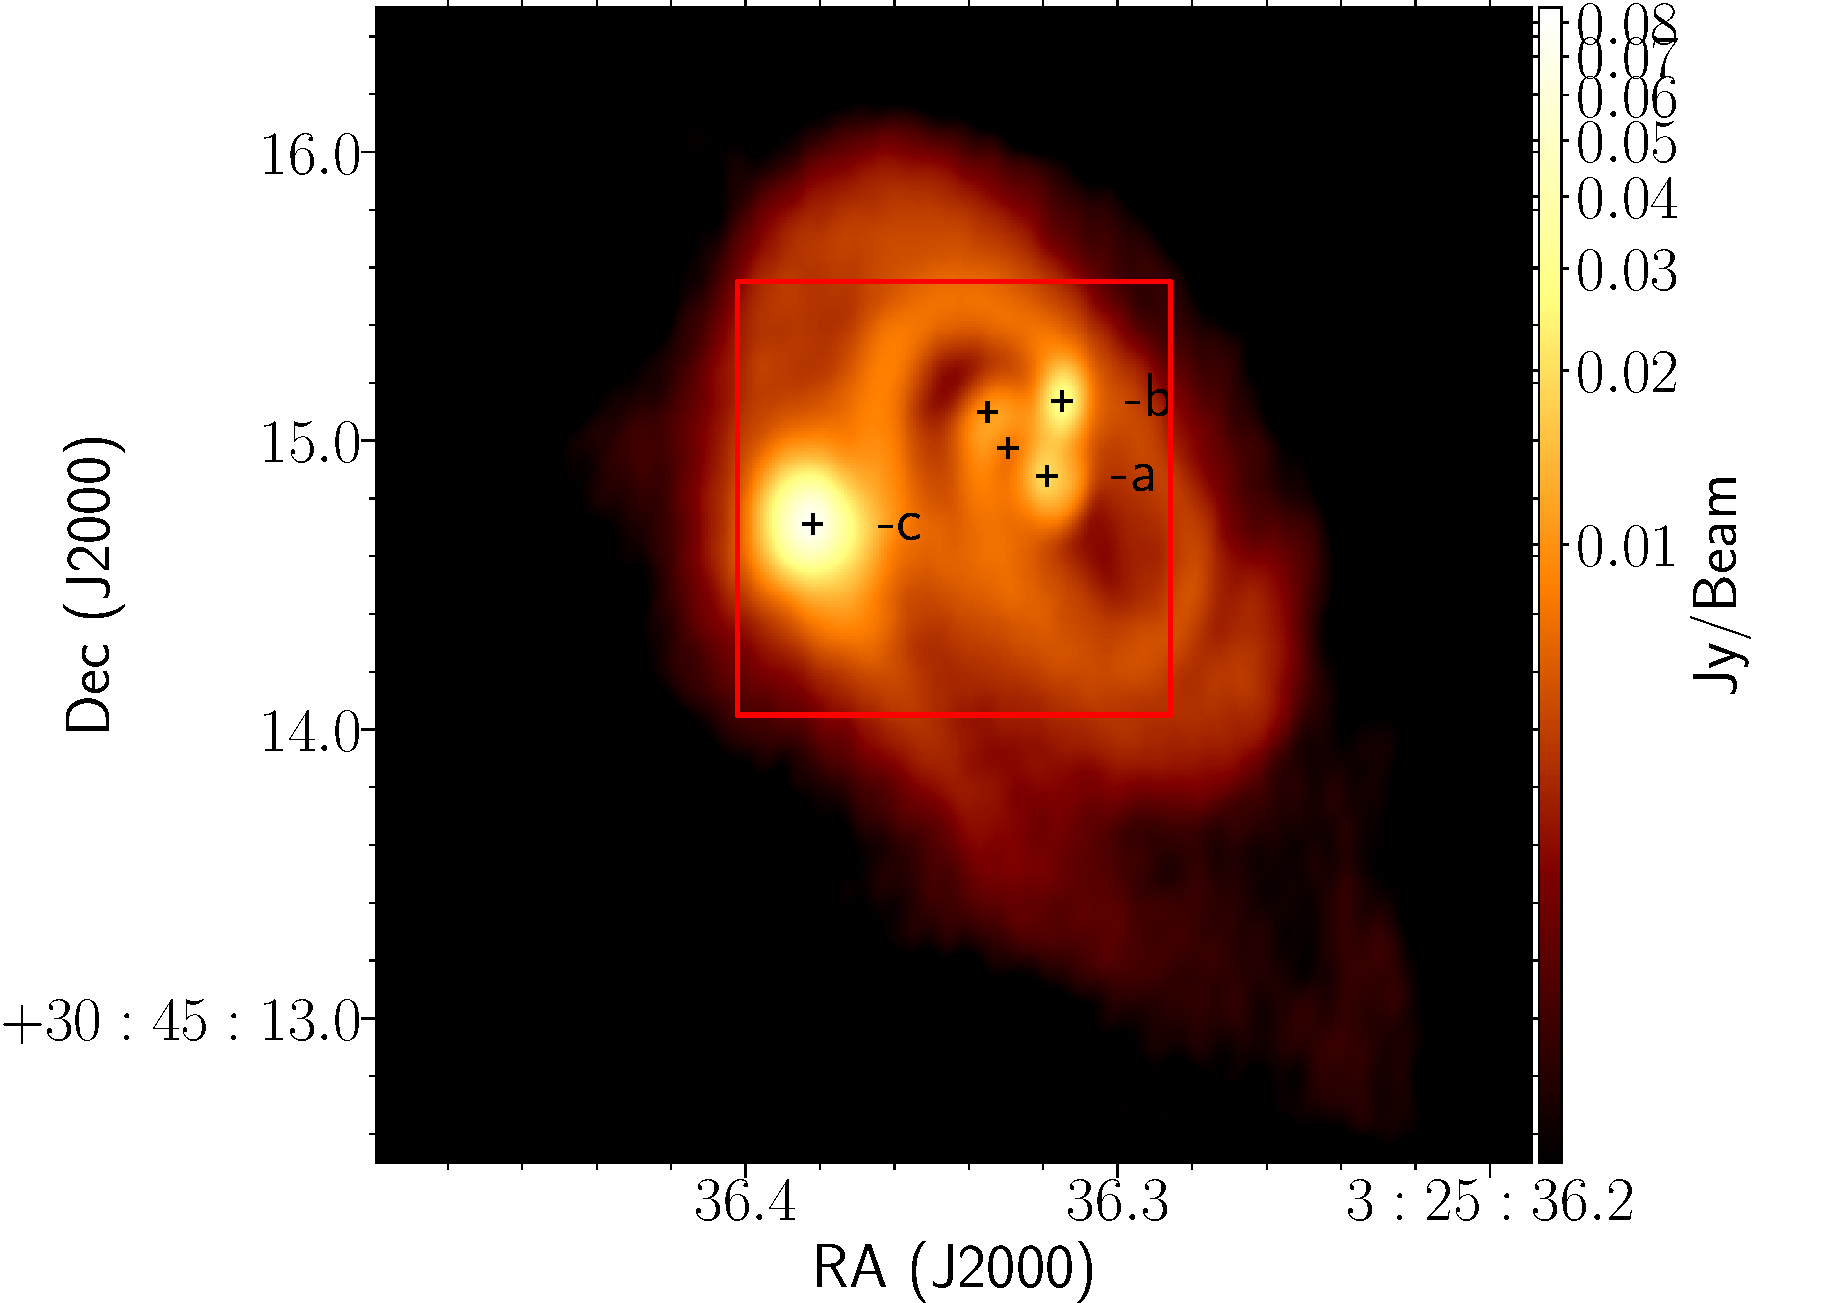
\includegraphics[width=0.49\textwidth]{img/L1448IRS3B_cont_robust05triplet_uc_forpos.pdf} % cont
   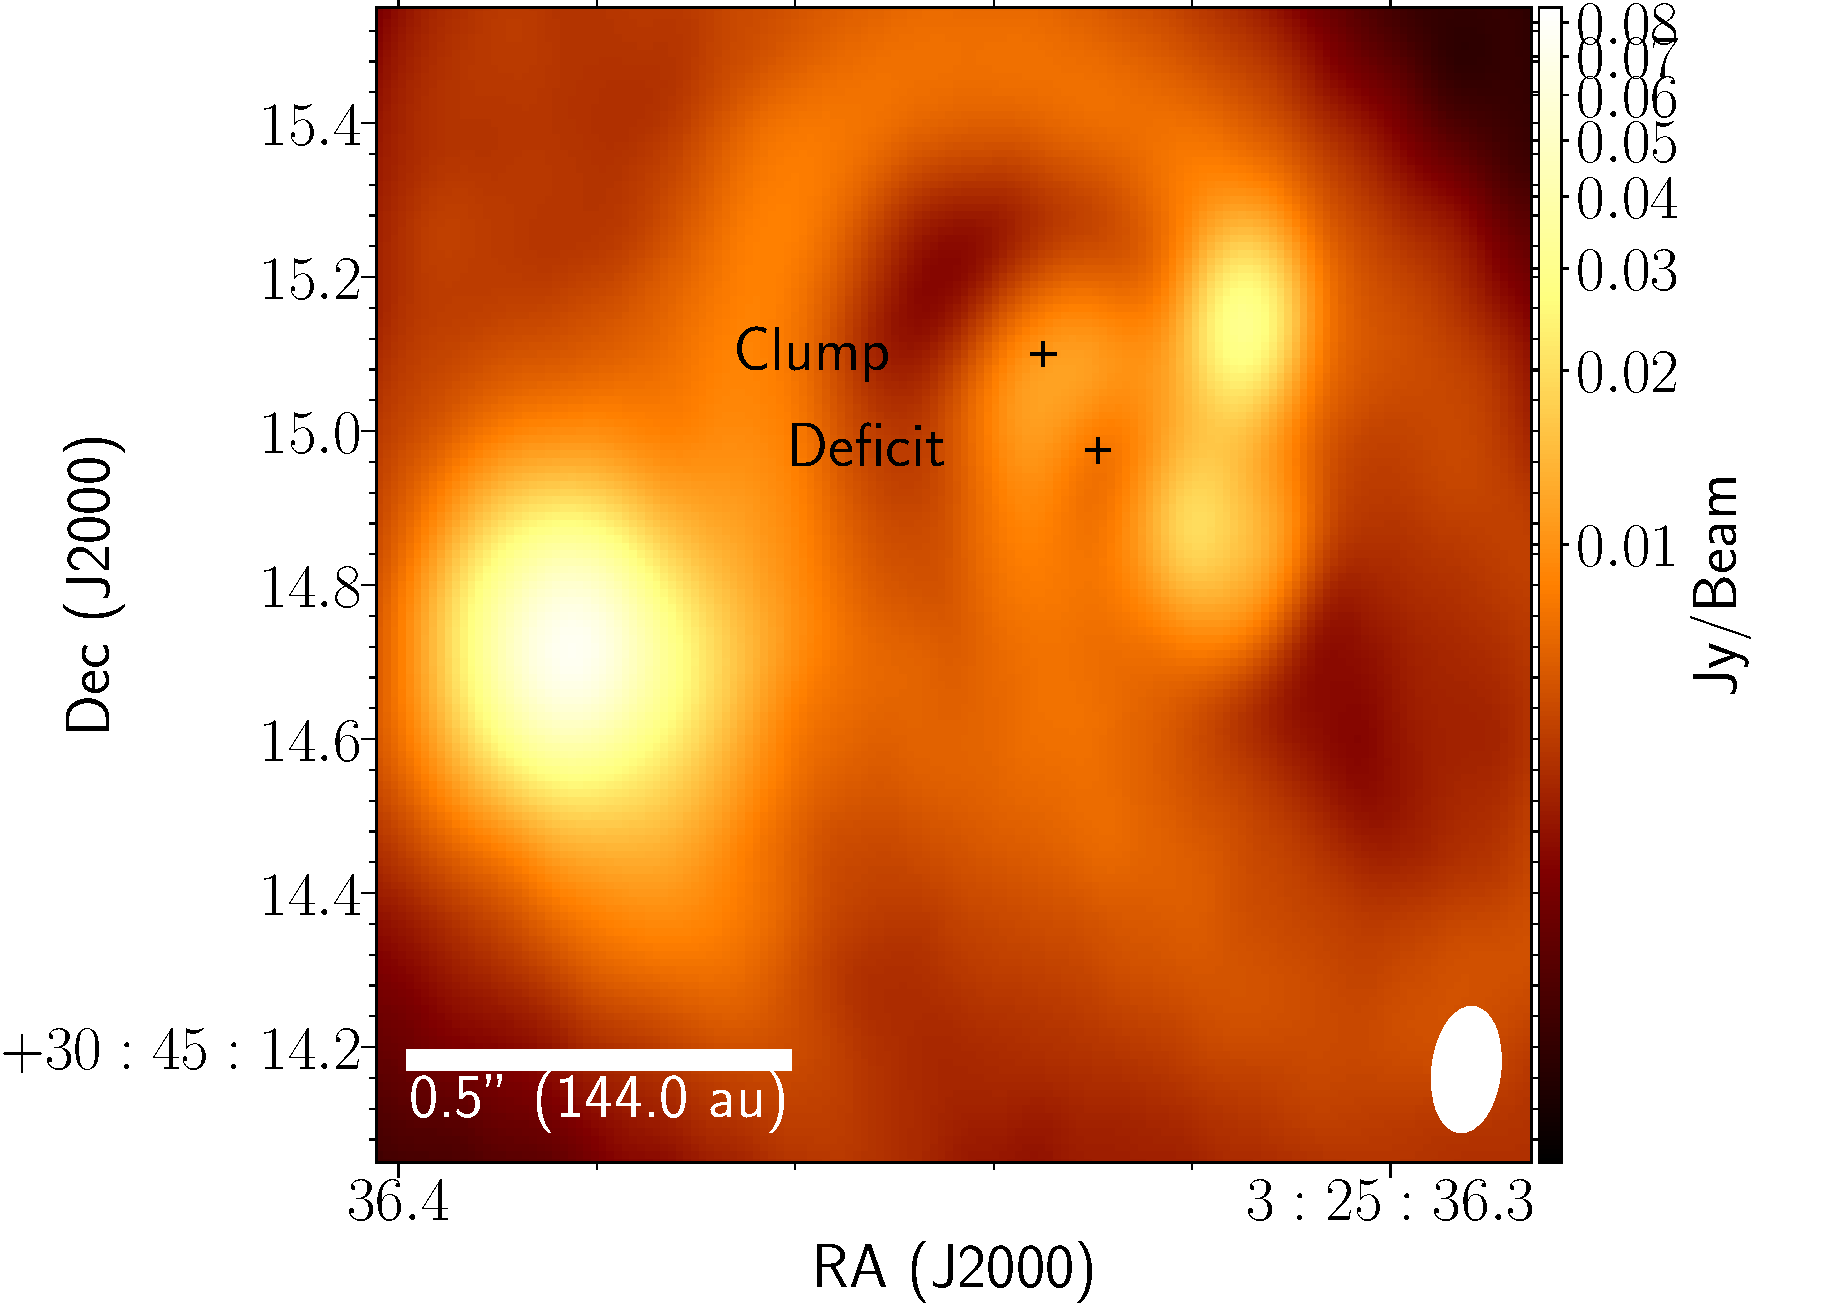
\includegraphics[width=0.49\textwidth]{img/L1448IRS3B_cont_robust05triplet_uc_positions.pdf} % cont
\end{center}
   \caption{ALMA 879~\micron\space continuum observations of the triple protostellar system L1448 IRS3B. The left colored image is zoomed in on IRS3B. The inner binary is separated by 0\farcs25 (75~AU) and has a circum-binary disk with spiral structure and the tertiary is separated from the binary by \ab0\farcs8 (230~AU) within one of the arms. The ``protostars'' are the continuum positions previously discovered in \citet{2016Natur.538..483T}, while the ``clump'' is a new feature, resolved in these observations. The ``deficit'' indicates the location of depression of flux between IRS3B-a and the ``clump''. This is discussed in Section~\ref{sec:dcont}. The beam size of each panel is shown in lower right (\contbeam\space using Briggs Robust parameter of 0.5).}\label{fig:zoomincont}
\end{figure}


\begin{figure}[H]
  \begin{center}
   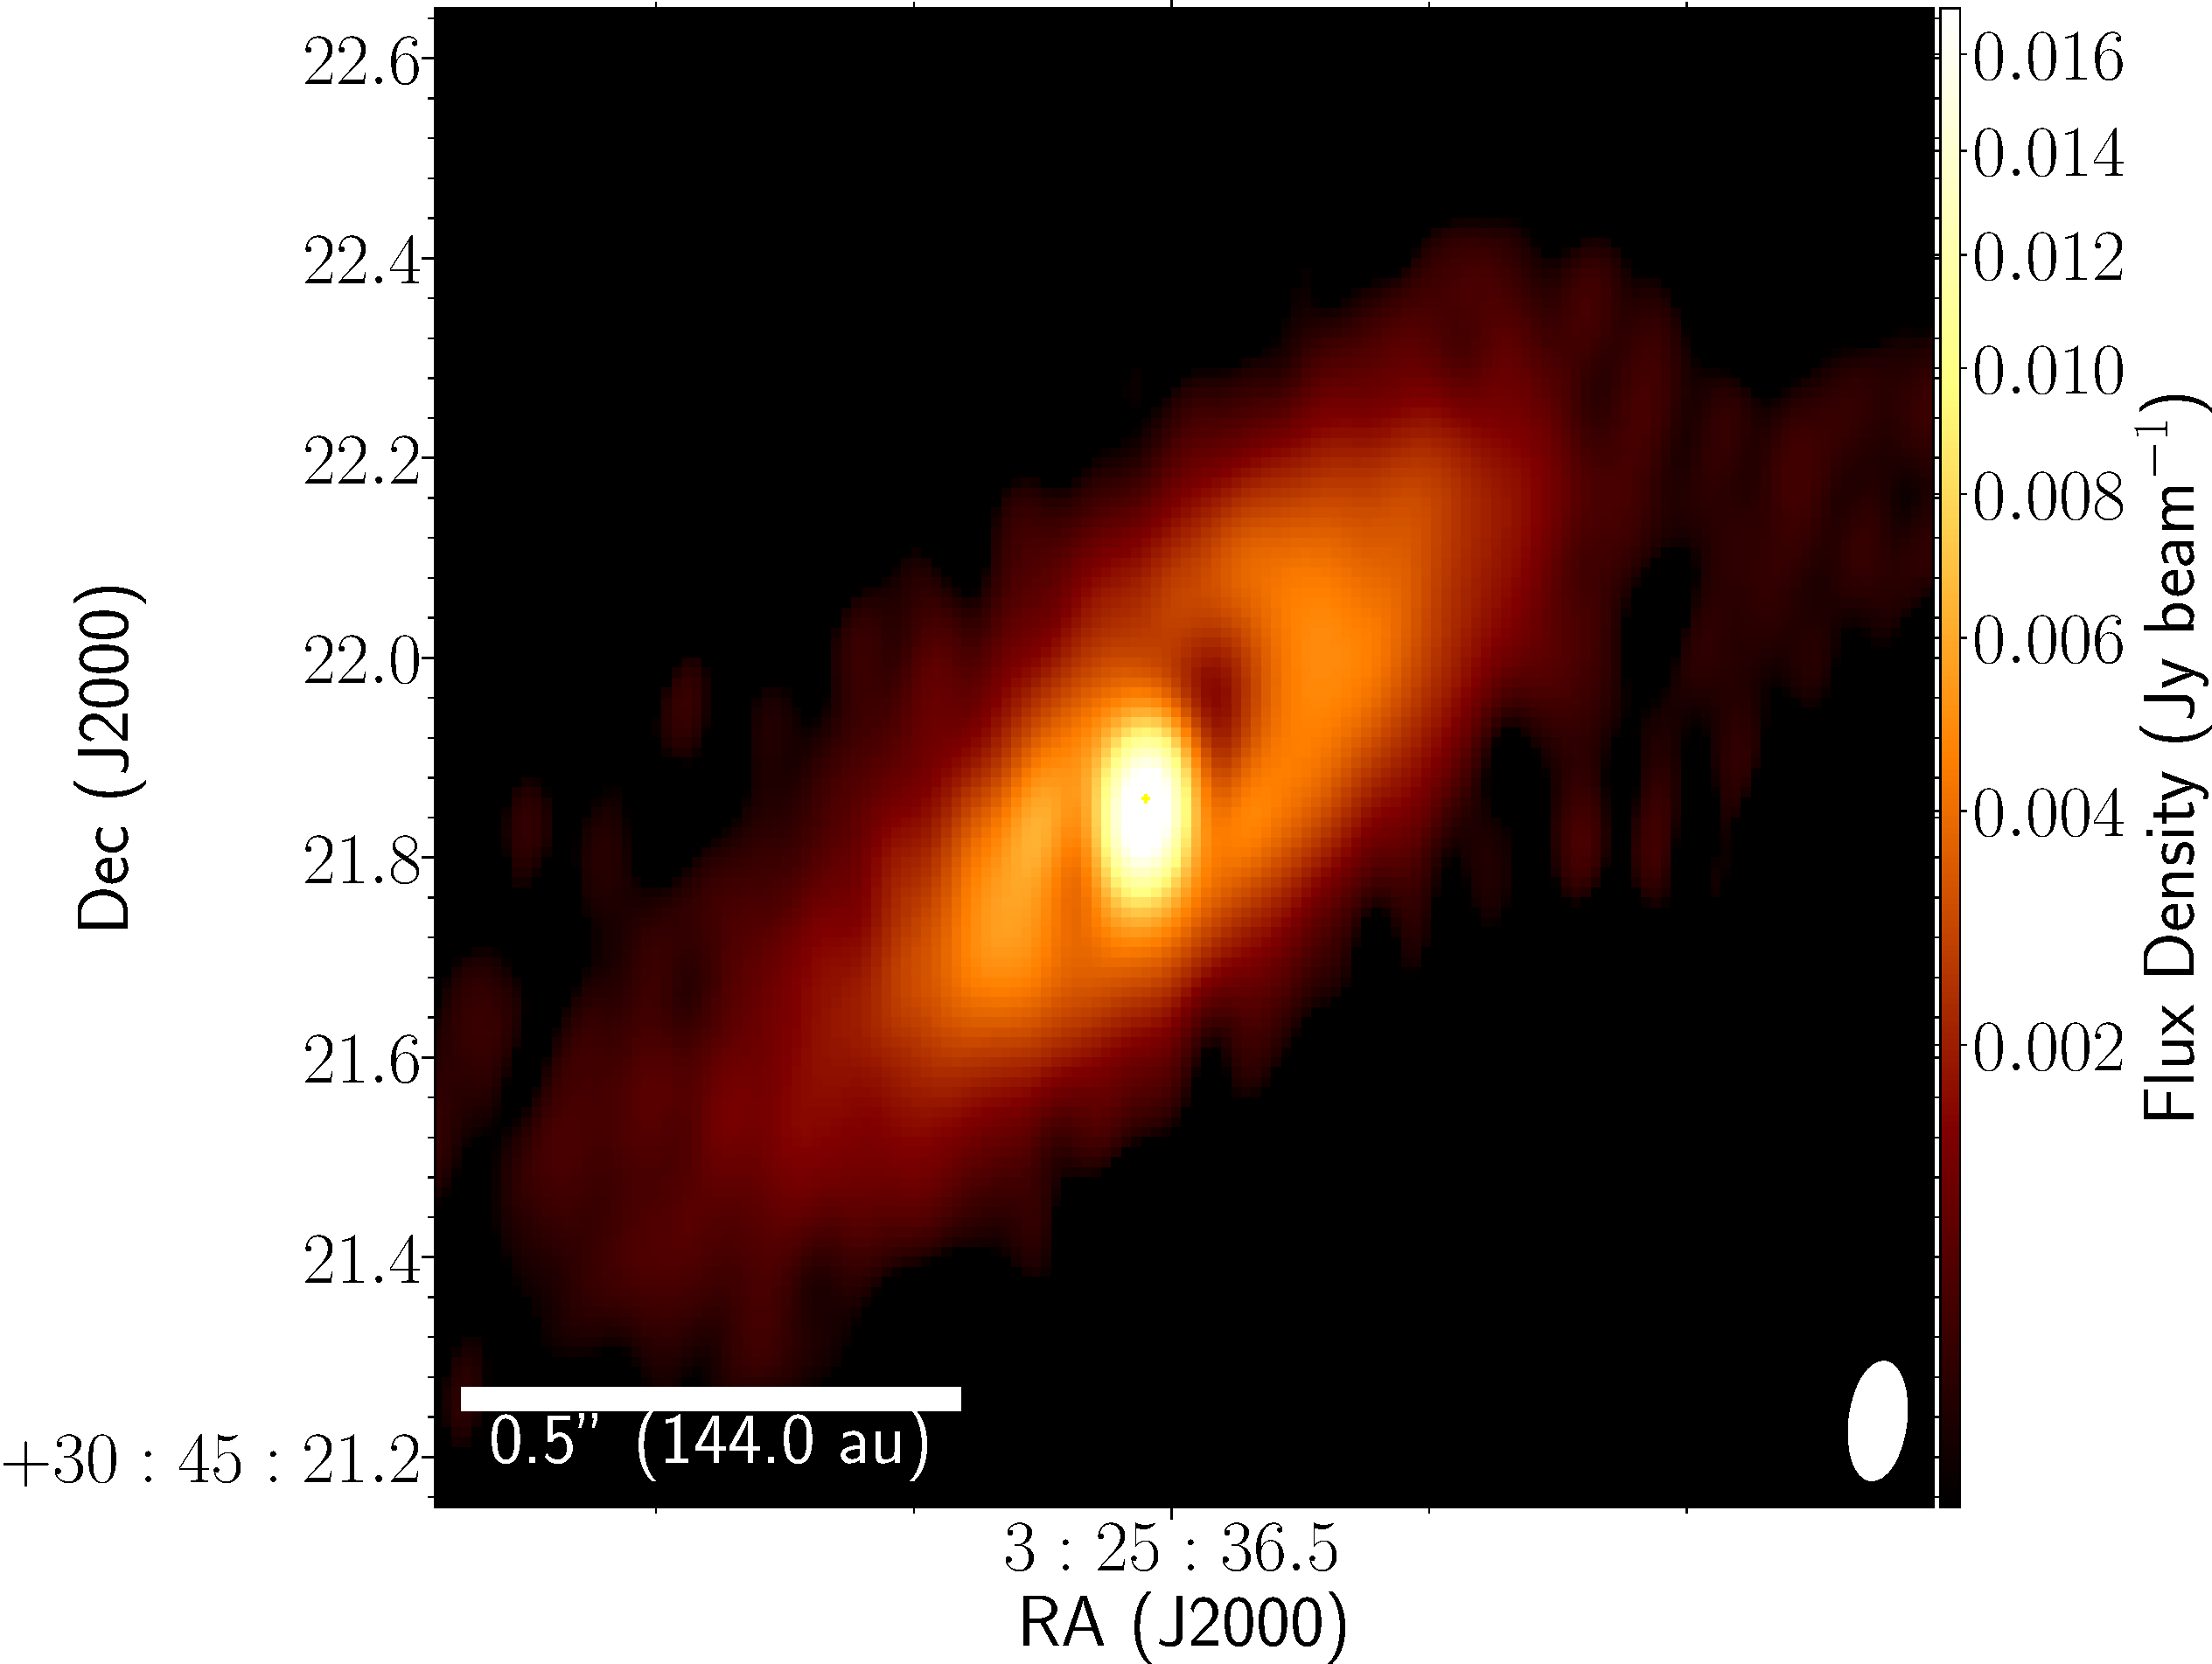
\includegraphics[width=0.48\textwidth]{img/L1448IRS3B-cont-irs3a-highres.pdf} % co
   \end{center}
   \caption{Continuum (879~\micron) image of IRS3A, reconstructed with the \textit{superuniform} weighing scheme, half of the cell size, and zoomed 2x from the images in Figure~\ref{fig:zoomincont}\space to highlight the possible spiral substructure.} \label{fig:widesuperuniform}
\end{figure}


% Figure 2
\begin{figure}[H]
\begin{center}
   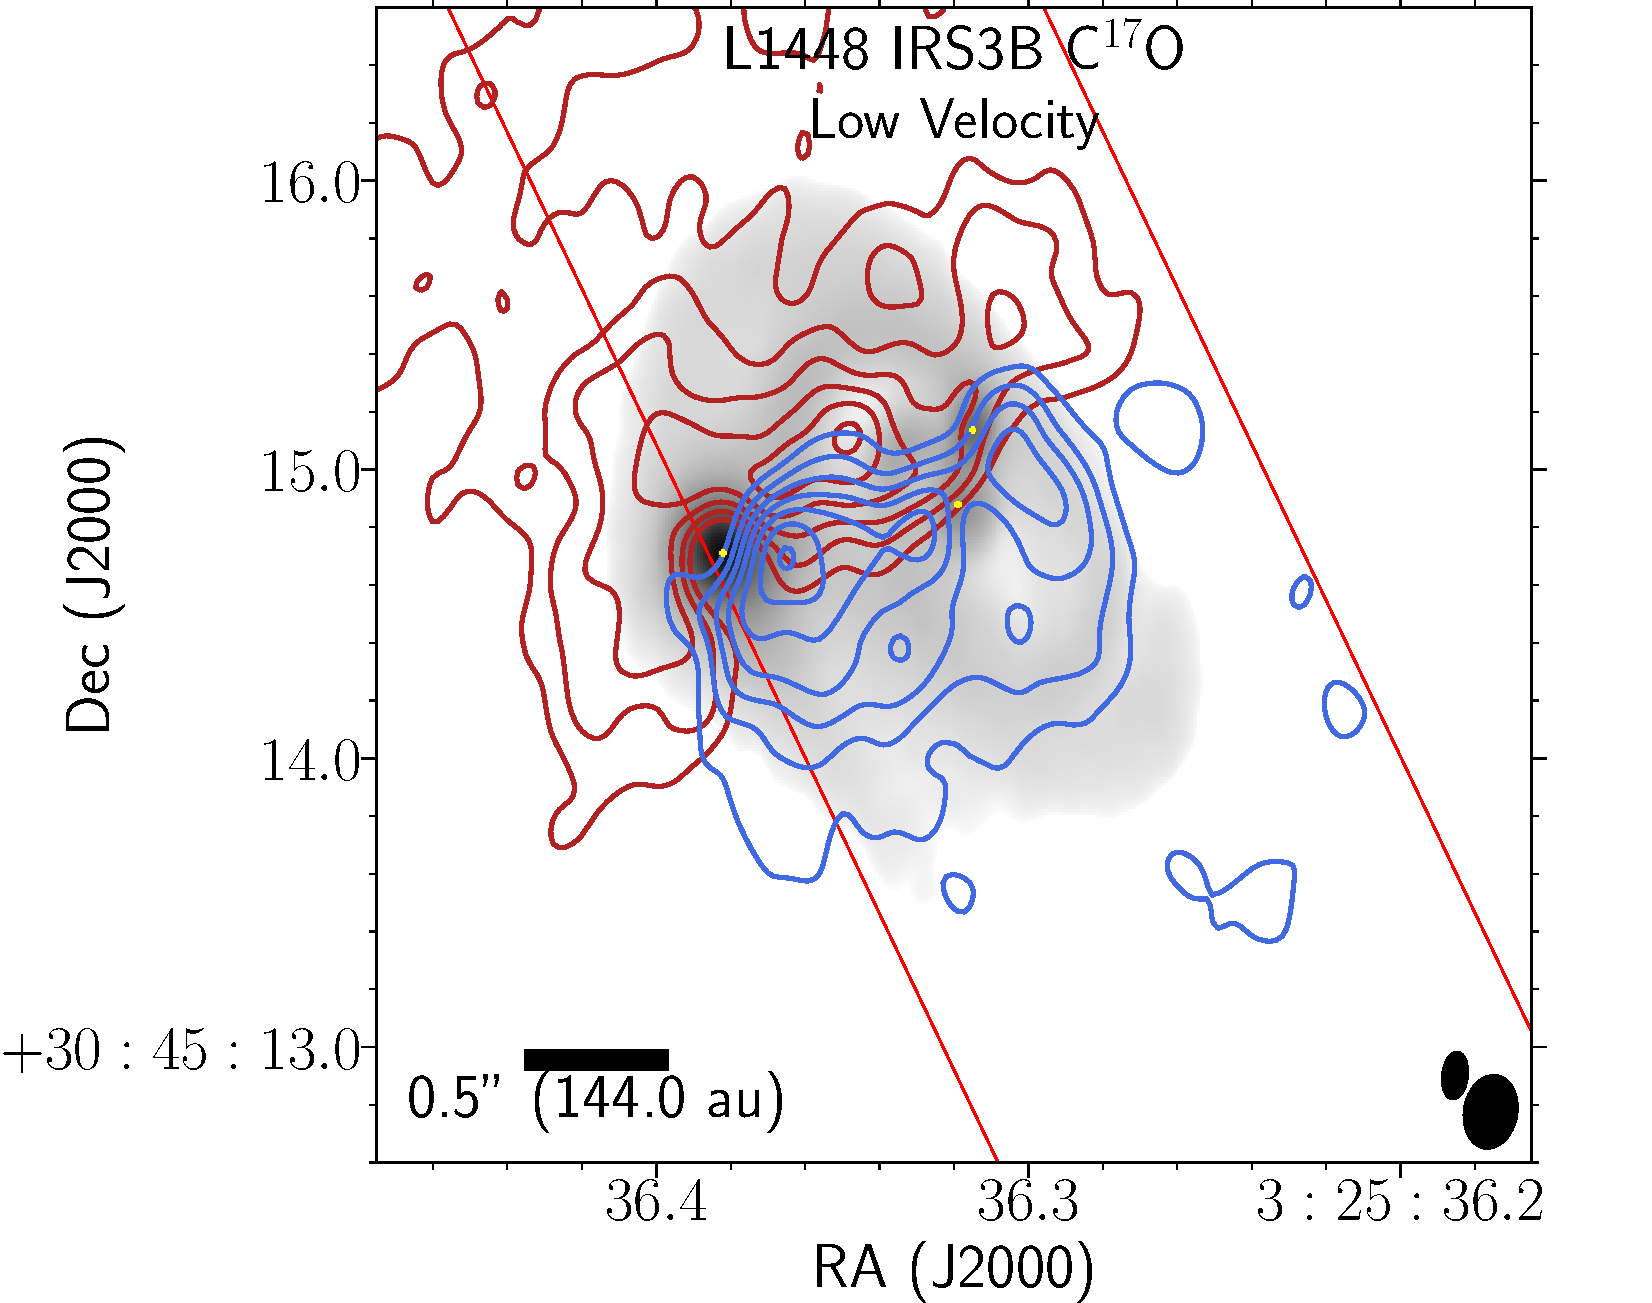
\includegraphics[width=0.33\textwidth]{img/L1448IRS3B_C17O_image_taper1500k__splitMoments_low.pdf} 
   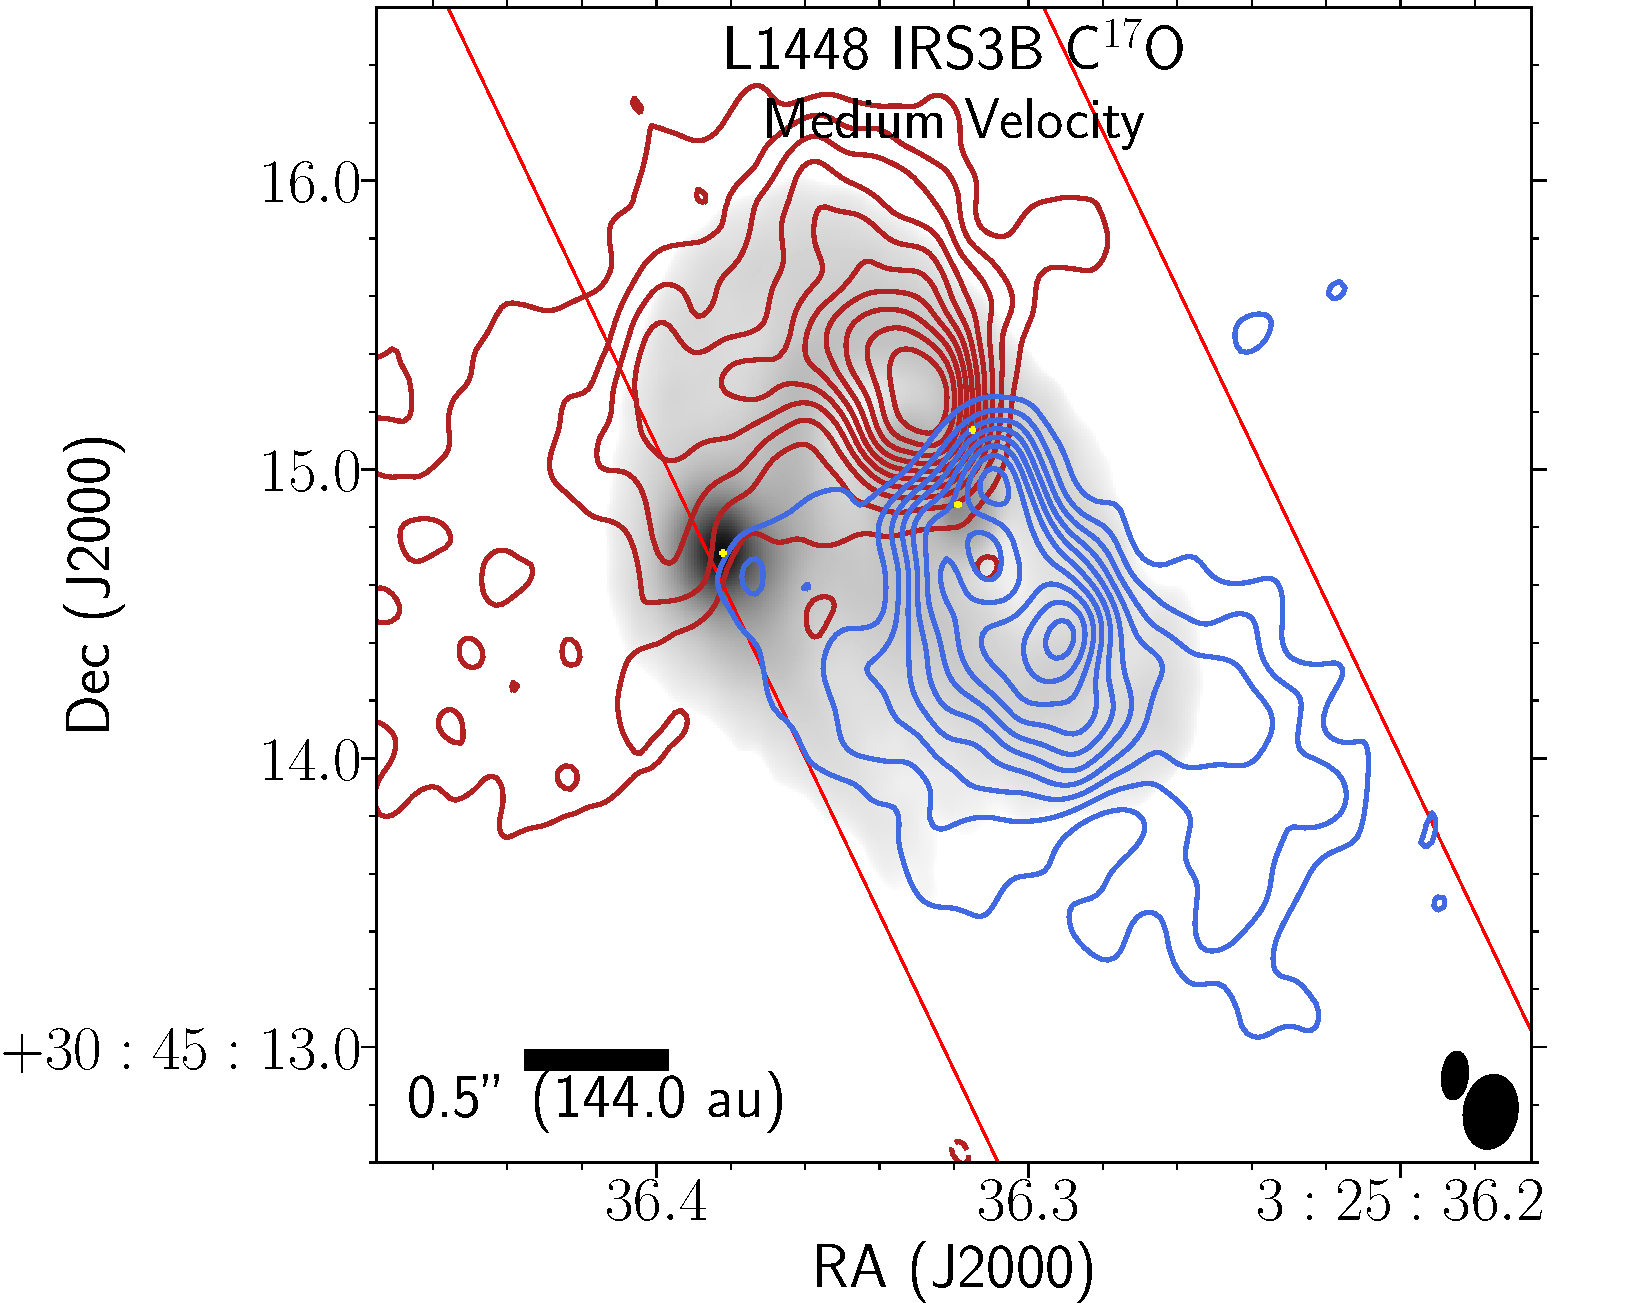
\includegraphics[width=0.33\textwidth]{img/L1448IRS3B_C17O_image_taper1500k__splitMoments_med.pdf} 
   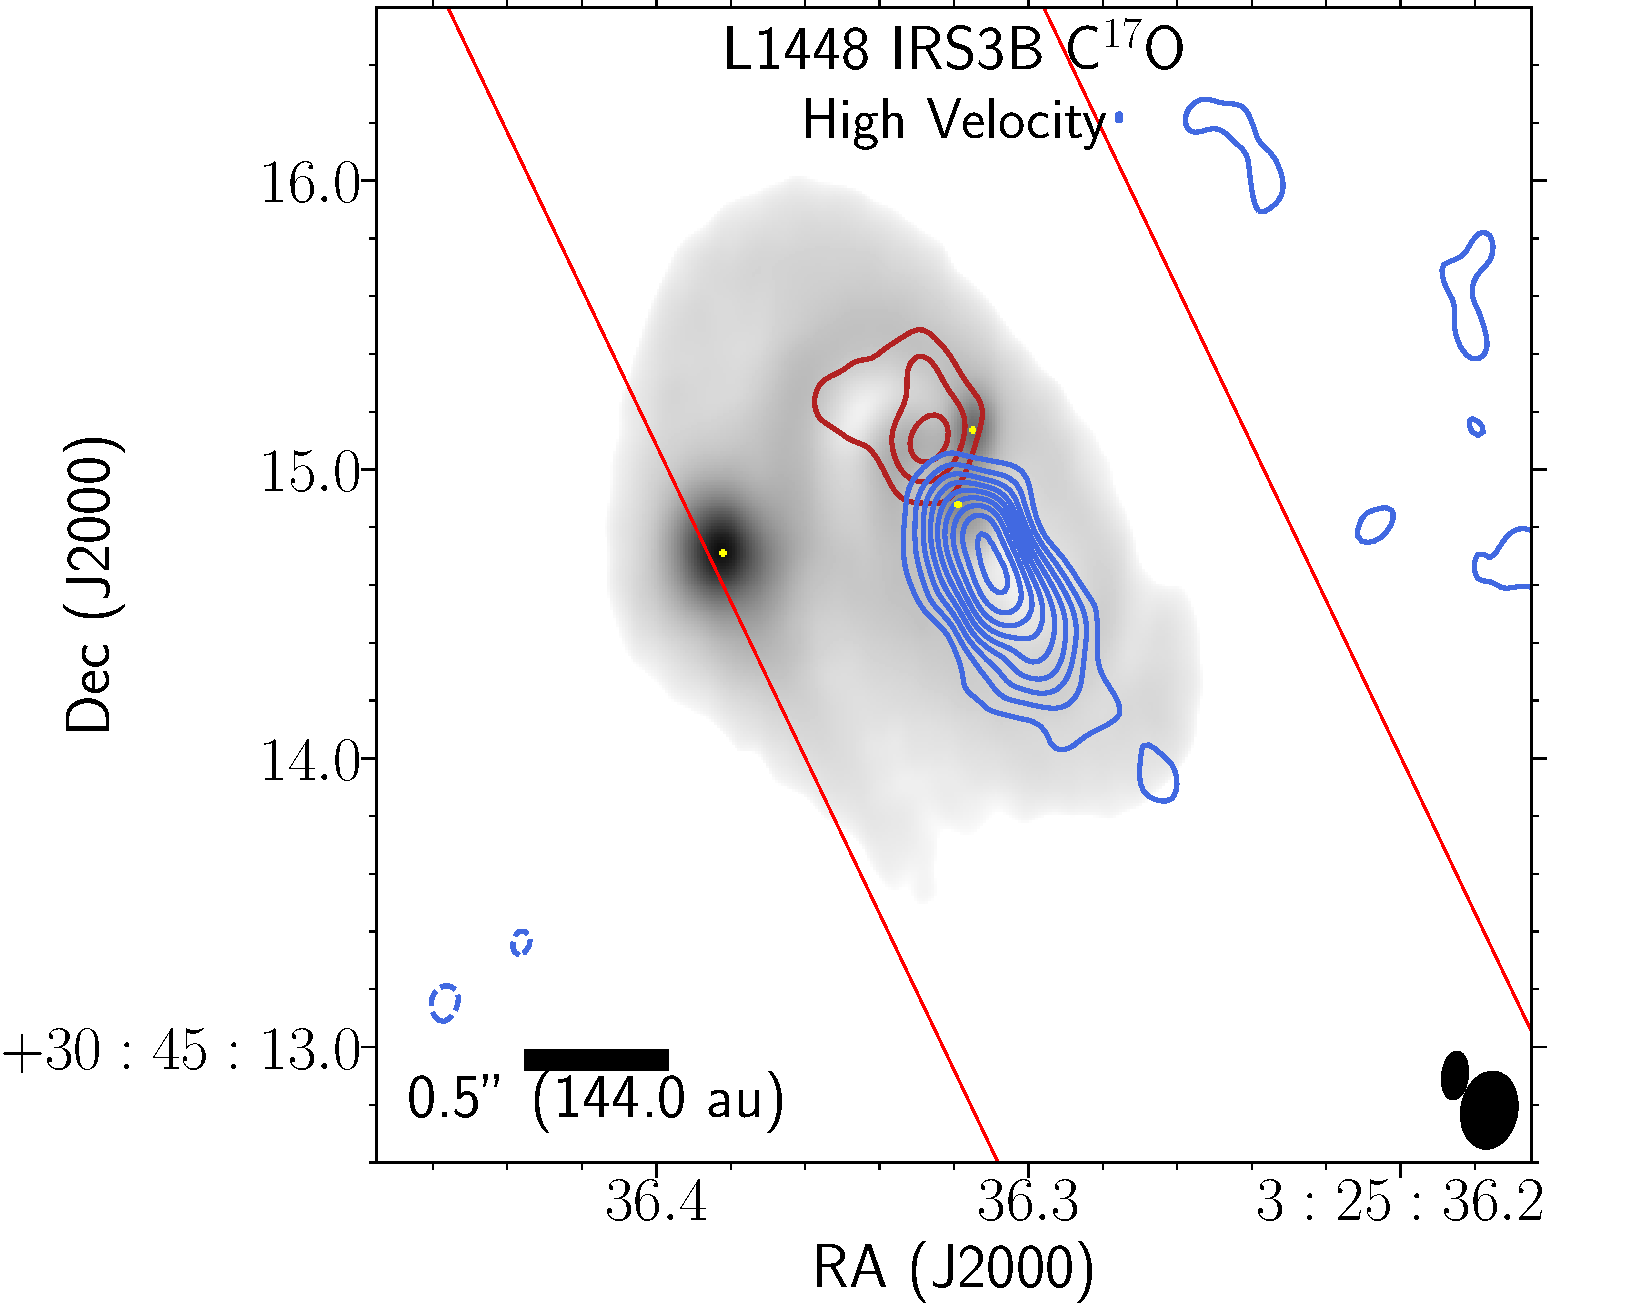
\includegraphics[width=0.33\textwidth]{img/L1448IRS3B_C17O_image_taper1500k__splitMoments_high.pdf}  % c17o
\end{center}
   \caption{\cso\space integrated intensity maps (herein moment 0 map) towards IRS3B over a selected range of velocities overlayed on continuum (grayscale). The \cso\space emission traces the rotating gas within the disk via Doppler-shifted emission. The panels correspond to low, medium, and high velocity ranges.% Negative contours are not present in these moment 0 maps; however, at the location of IRS3B-c, there is strong absorption that is evident in the high spectral resolution data cube, but is not represented here. 
   The red lines indicate the region extracted for PV diagram, along the position angle of the major axis. \textbf{Low Velocity:} Velocity range starts at 4.68$\rightarrow$5.67~\kms (3.58$\rightarrow$4.68~\kms) and contours start at 8(8)$\sigma$ and iterate by 3(3)$\sigma$ with the 1$\sigma$~level starting at 0.0023(0.0025)~Jy~beam$^{-1}$ for the red(blue) channels respectively. \textbf{Medium Velocity:} Velocity range starts at 5.67$\rightarrow$6.66~\kms (2.48$\rightarrow$3.58~\kms) and contours start at 3(5)$\sigma$ and iterate by 3(3)$\sigma$ with the 1$\sigma$~level starting at 0.002(0.0016)~Jy~beam$^{-1}$ for the red(blue) channels respectively. \textbf{High Velocity:} Velocity range starts at 6.66$\rightarrow$7.65~\kms (1.27$\rightarrow$2.48~\kms) and contours start at 5(5)$\sigma$ and iterate by 3(3)$\sigma$ with the 1$\sigma$~level starting at 0.0018(0.0012)~Jy~beam$^{-1}$ for the red(blue) channels respectively. The \cso\space synthesized beam (\csobeam) is the bottom-right most ellipse on each of the panels and the continuum synthesized beam (\contbeam) is offset diagonally.}\label{fig:irs3bc17omoment}
\end{figure}




% Figure 8
% irs3a
\begin{figure}[H]
\begin{center}
   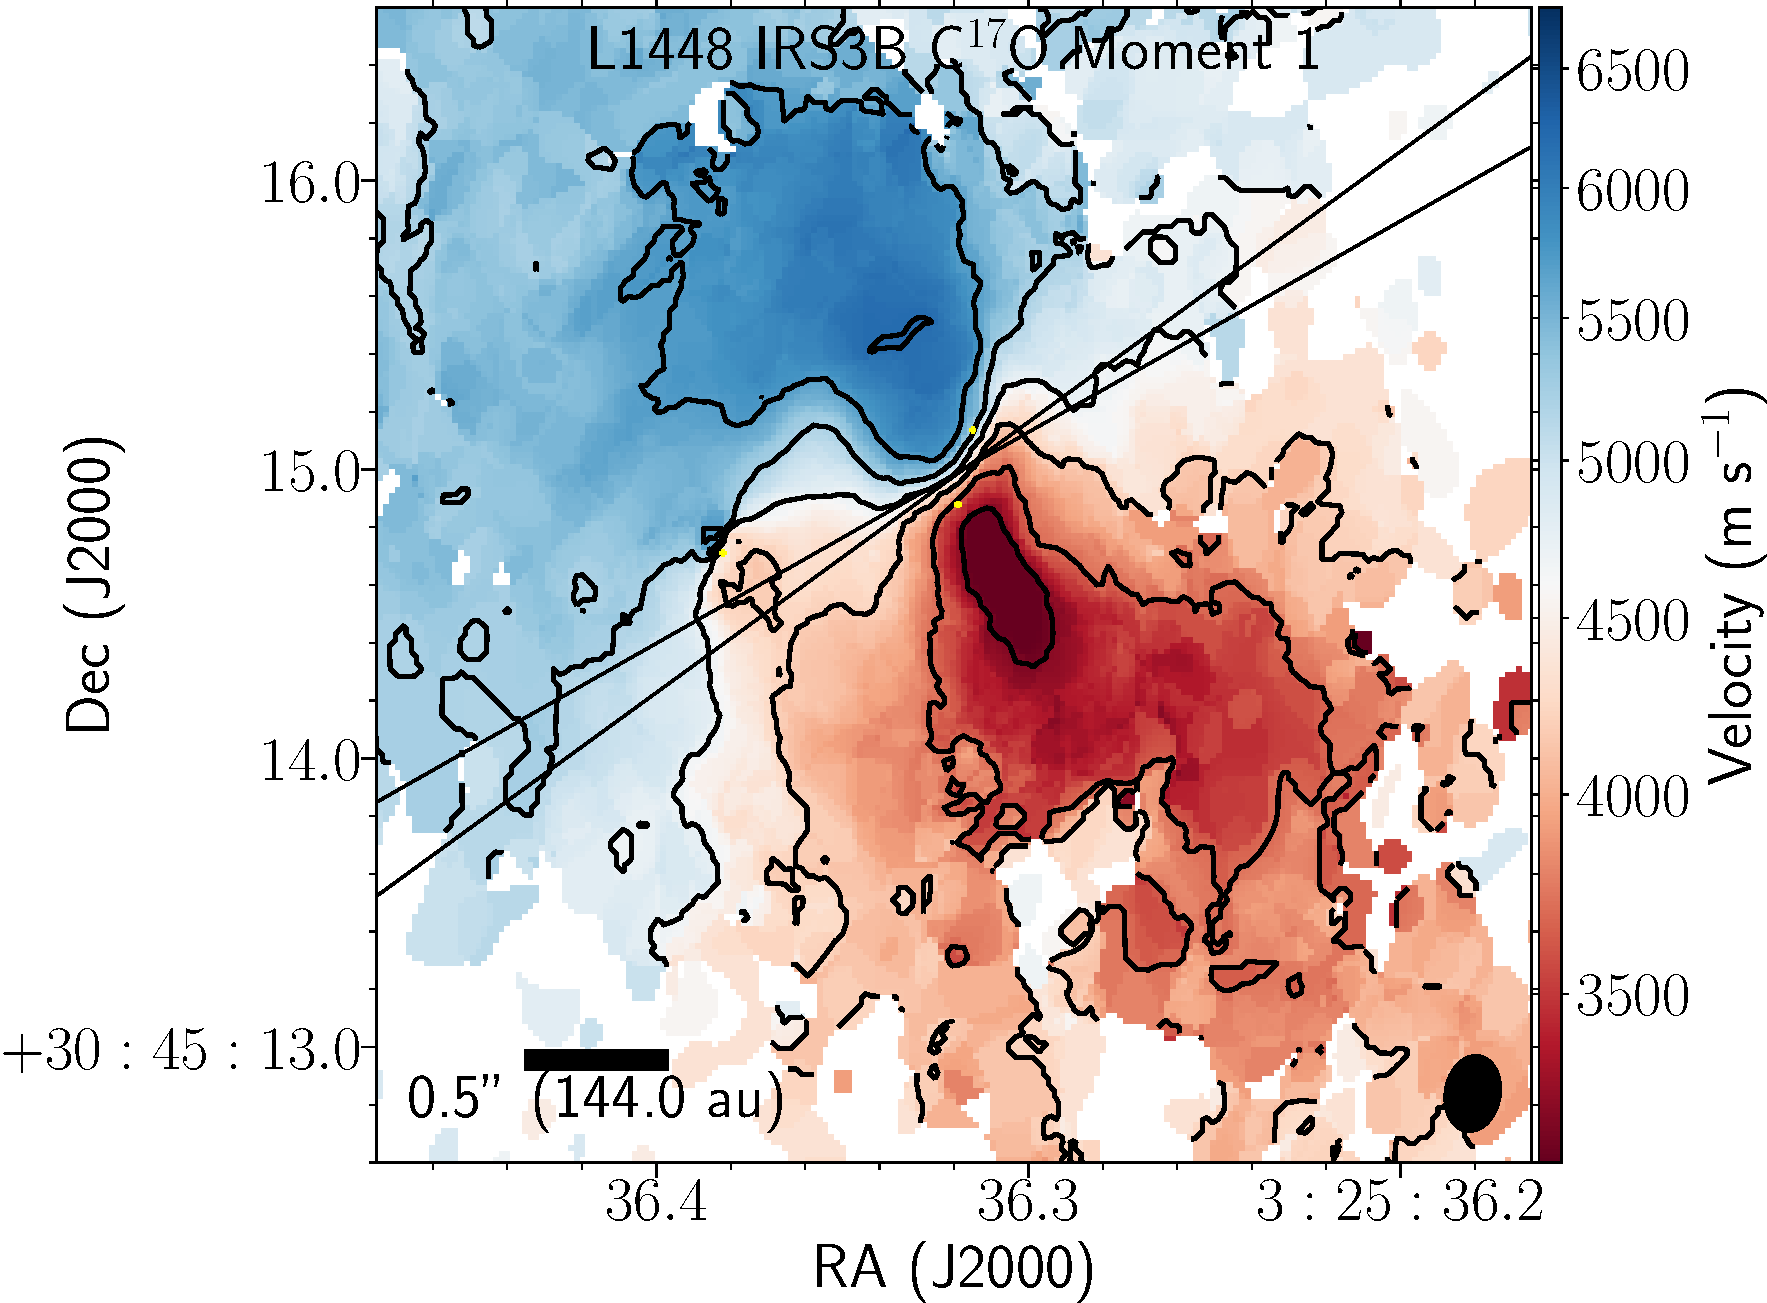
\includegraphics[width=0.5\textwidth]{img/L1448IRS3B_C17O_image_taper1500k_image_M1_fits.pdf}  % c17o
\end{center}
   \caption{\cso\space velocity-weighted moment 1 maps toward IRS3B over a selected range of velocities (1.27$\rightarrow$7.65~\kms) The \cso\space emission appears well ordered across the semi-major axis. The contours denote the 0.5~km~s$^{-1}$ velocity offsets from system velocity of 4.8~km~s$^{-1}$. The yellow markers indicate the three continuum sources. The black lines indicate the position angle of the minor disk estimates as given by the \pdspy\space fitting routine in Table~\ref{table:pvtable}, of $90+26.7^{+  1.8}_{-  2.9}$\deg. The \cso\space synthesized beam (\csobeam) is the bottom-right most ellipse.}\label{fig:irs3abc17omoment1}
\end{figure}

% figure will go here for pv cutout, 2 of them




% Figure 10
\begin{figure}[H]
\begin{center}
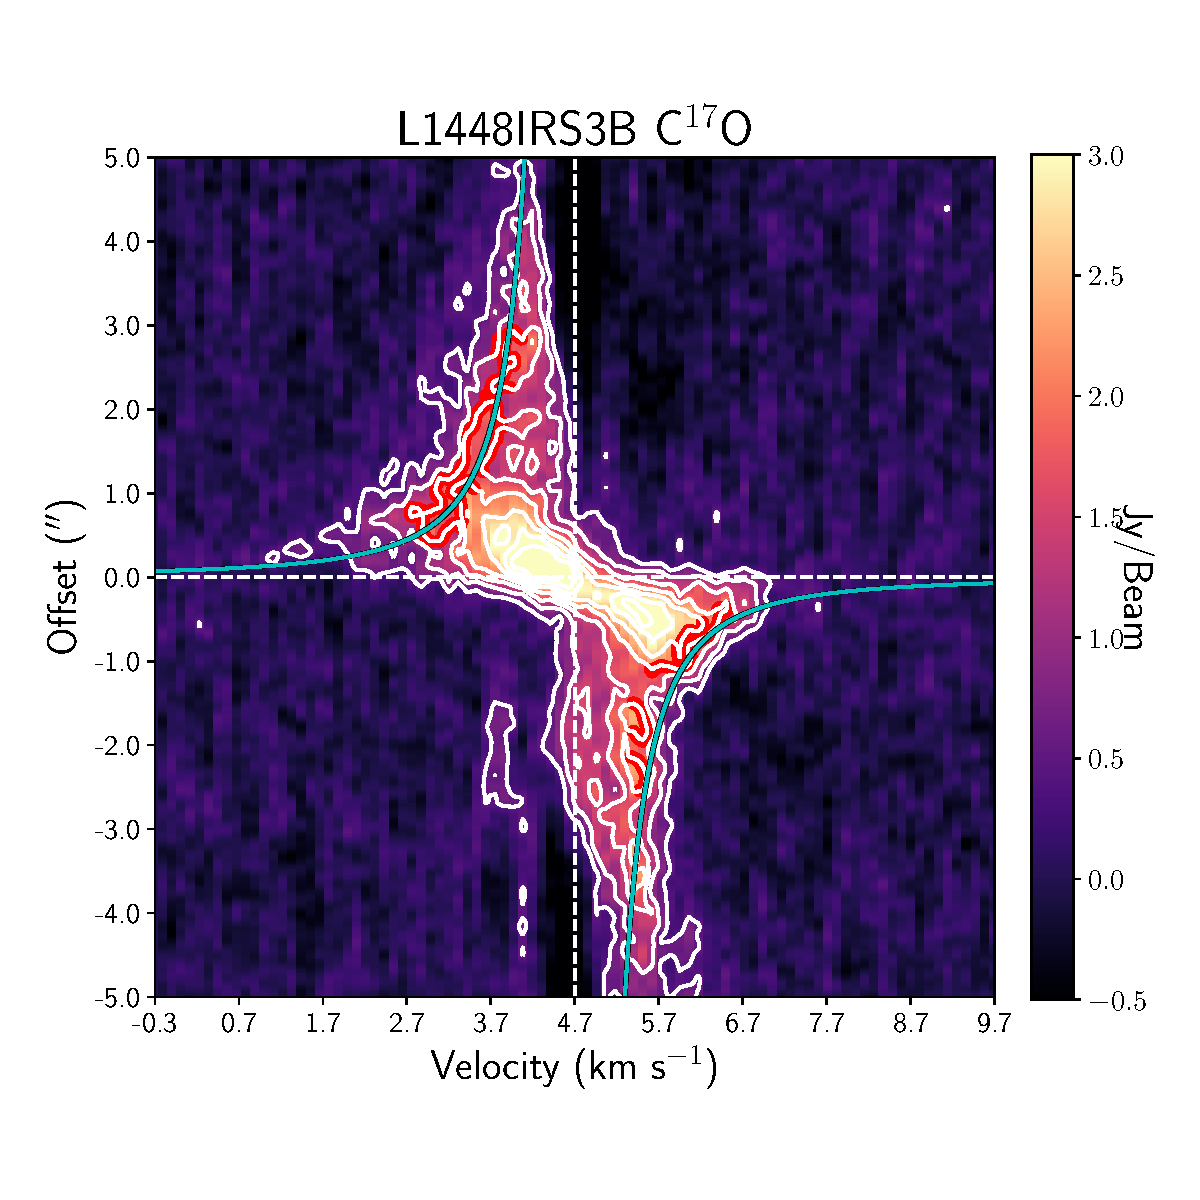
\includegraphics[width=0.49\textwidth]{img/irs3b_c17o_pv.pdf}
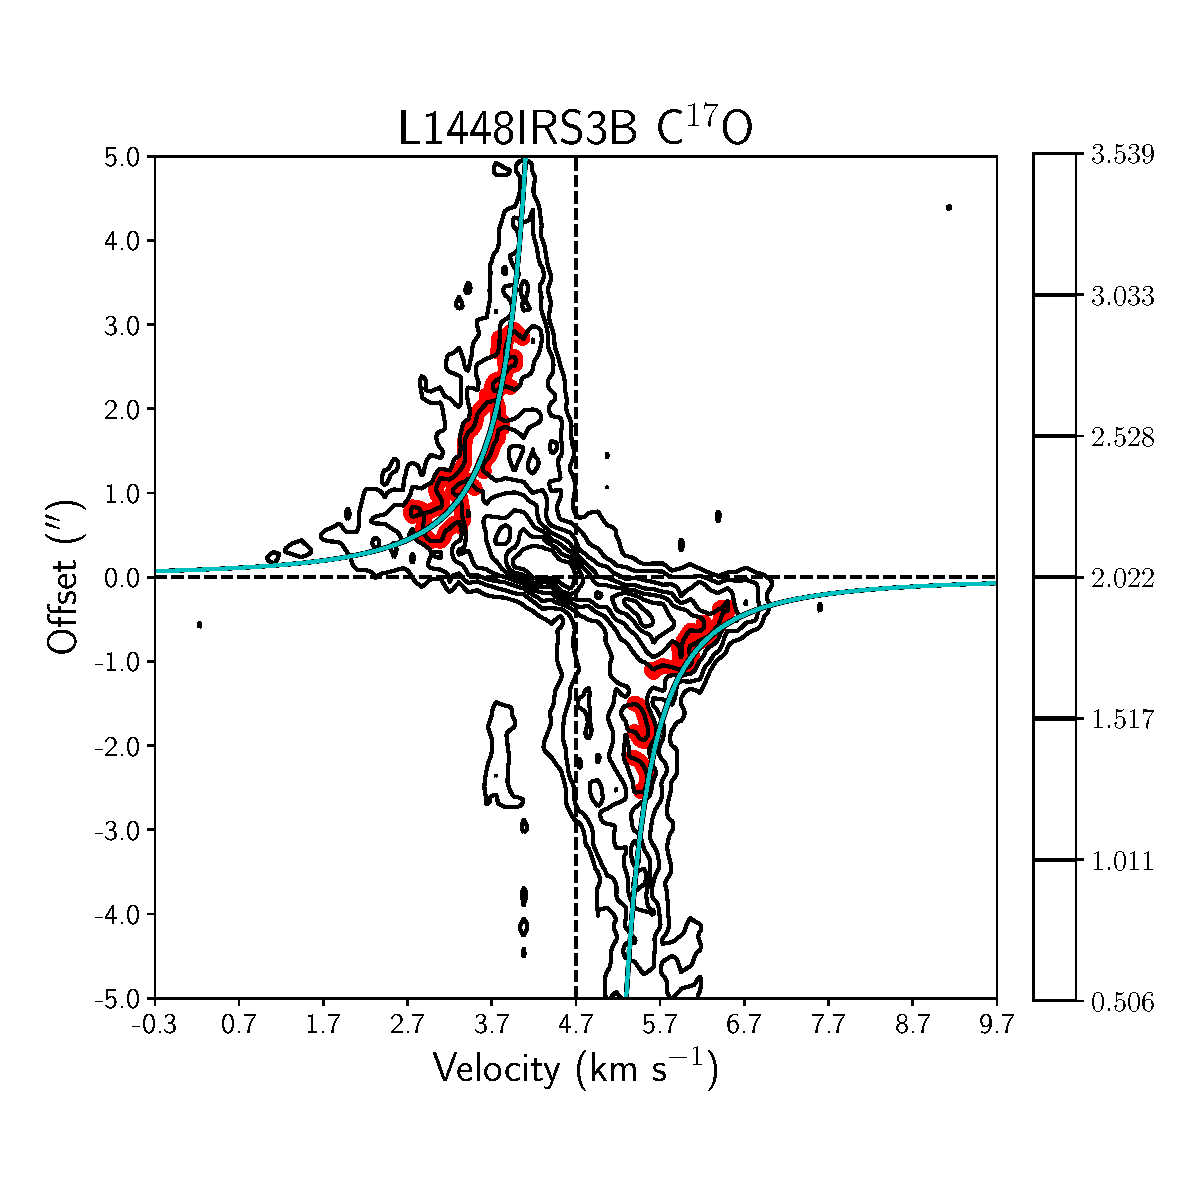
\includegraphics[width=0.49\textwidth]{img/PV-Diagram_L1448IRS3B_C17O_image_taper1500k_fit_xtr.pdf}
%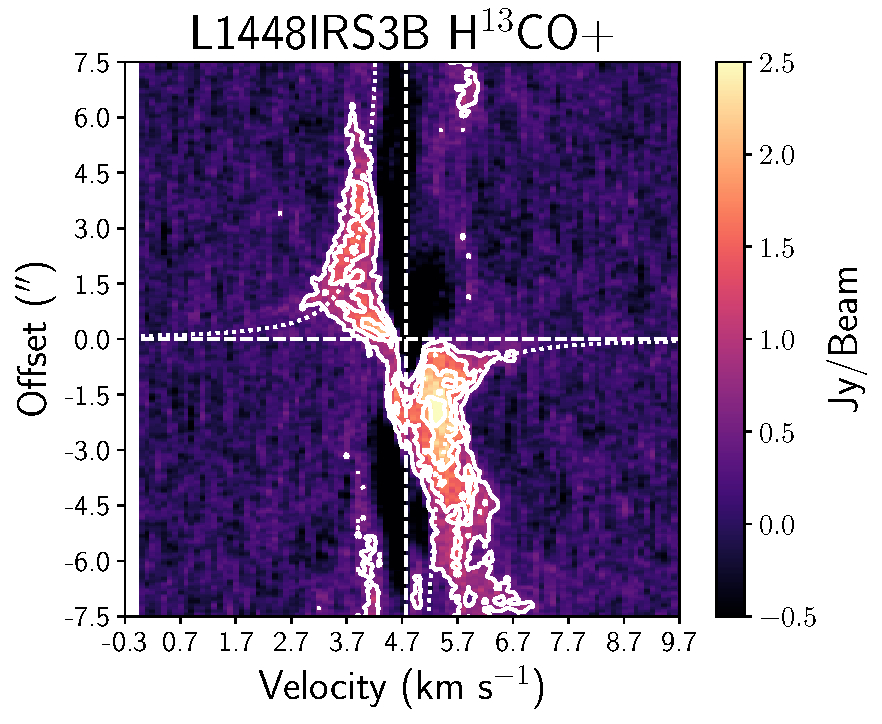
\includegraphics[width=0.33\textwidth]{img/PV-Diagram_L1448IRS3B_H13COp_image_taper1500k.pdf}
\end{center}
\caption{PV-diagrams of IRS3B generated at a position angle of 29\deg. \cso\space (left, middle) emission with the cyan lines corresponding to the fit of 1.15~\solm. The cyan line traces the median fit for numeric Keplerian orbital fit routine while the black lines represent 100 randomly sampled MCMC fits, used to estimate errors. The white/black contours trace regions starting from 3$\sigma$ at 2$\sigma$\space intervals, where $\sigma\approx$0.14~Jy~beam$^{-1}$. The red contours trace the regions selected for the MCMC fit which are defined as the 10 and 12$\sigma$. \htcop\space (right) demonstrates the data are not inconsistent with a 1.15~\solm\space protostar, however the emission is largely asymmetric and coupled with the envelope. The white contours trace regions starting from 3$\sigma$ at 2$\sigma$\space intervals, where $\sigma\approx$0.15~Jy.}\label{fig:l1448irs3b_c17o_pv}
\end{figure}




% Figure 7
\begin{figure}[H]
\begin{center}
   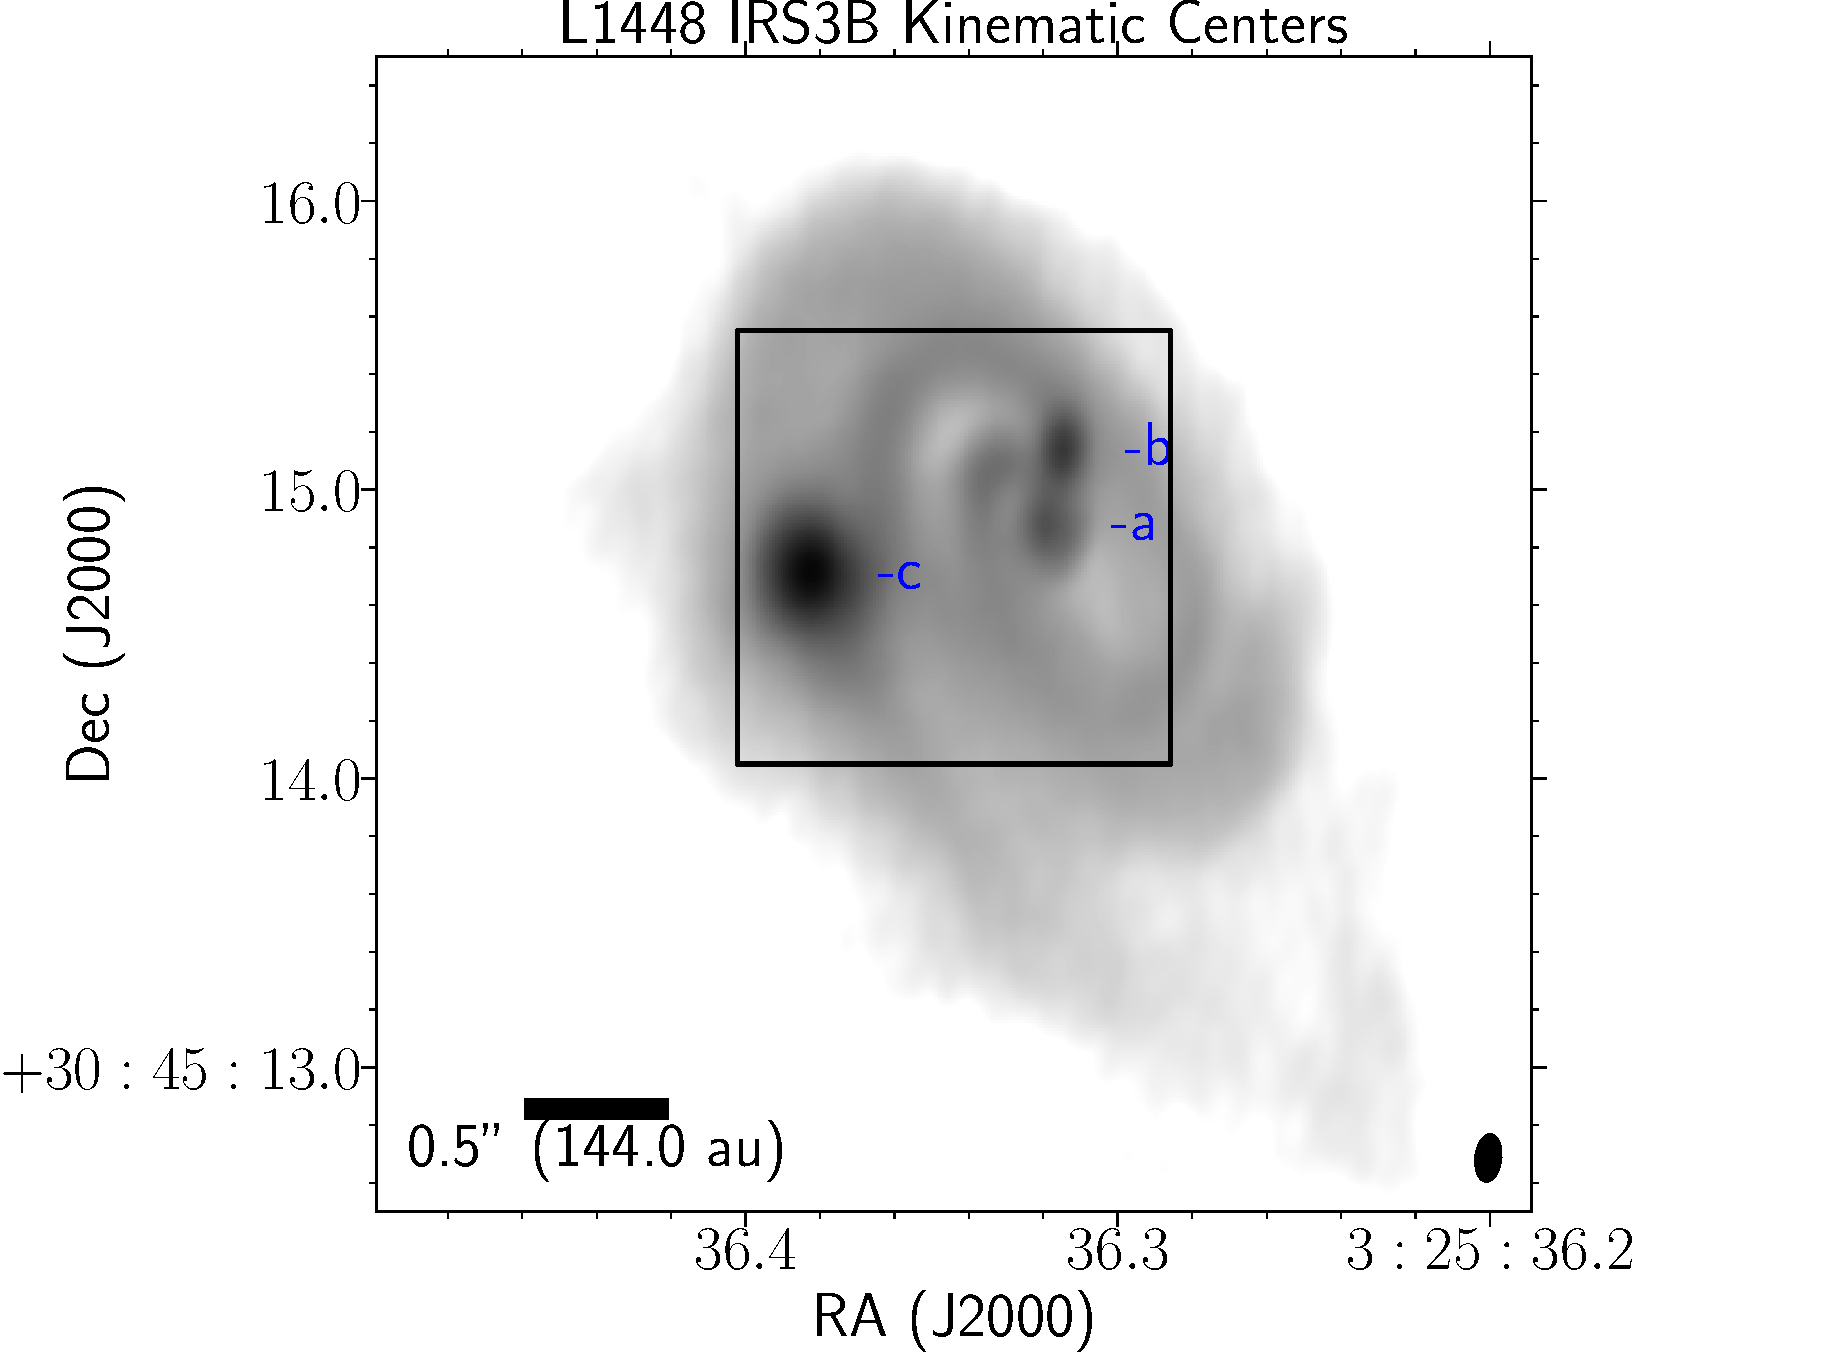
\includegraphics[width=0.48\textwidth]{img/L1448IRS3B_cont_robust05kincenters.pdf} % h13cn
   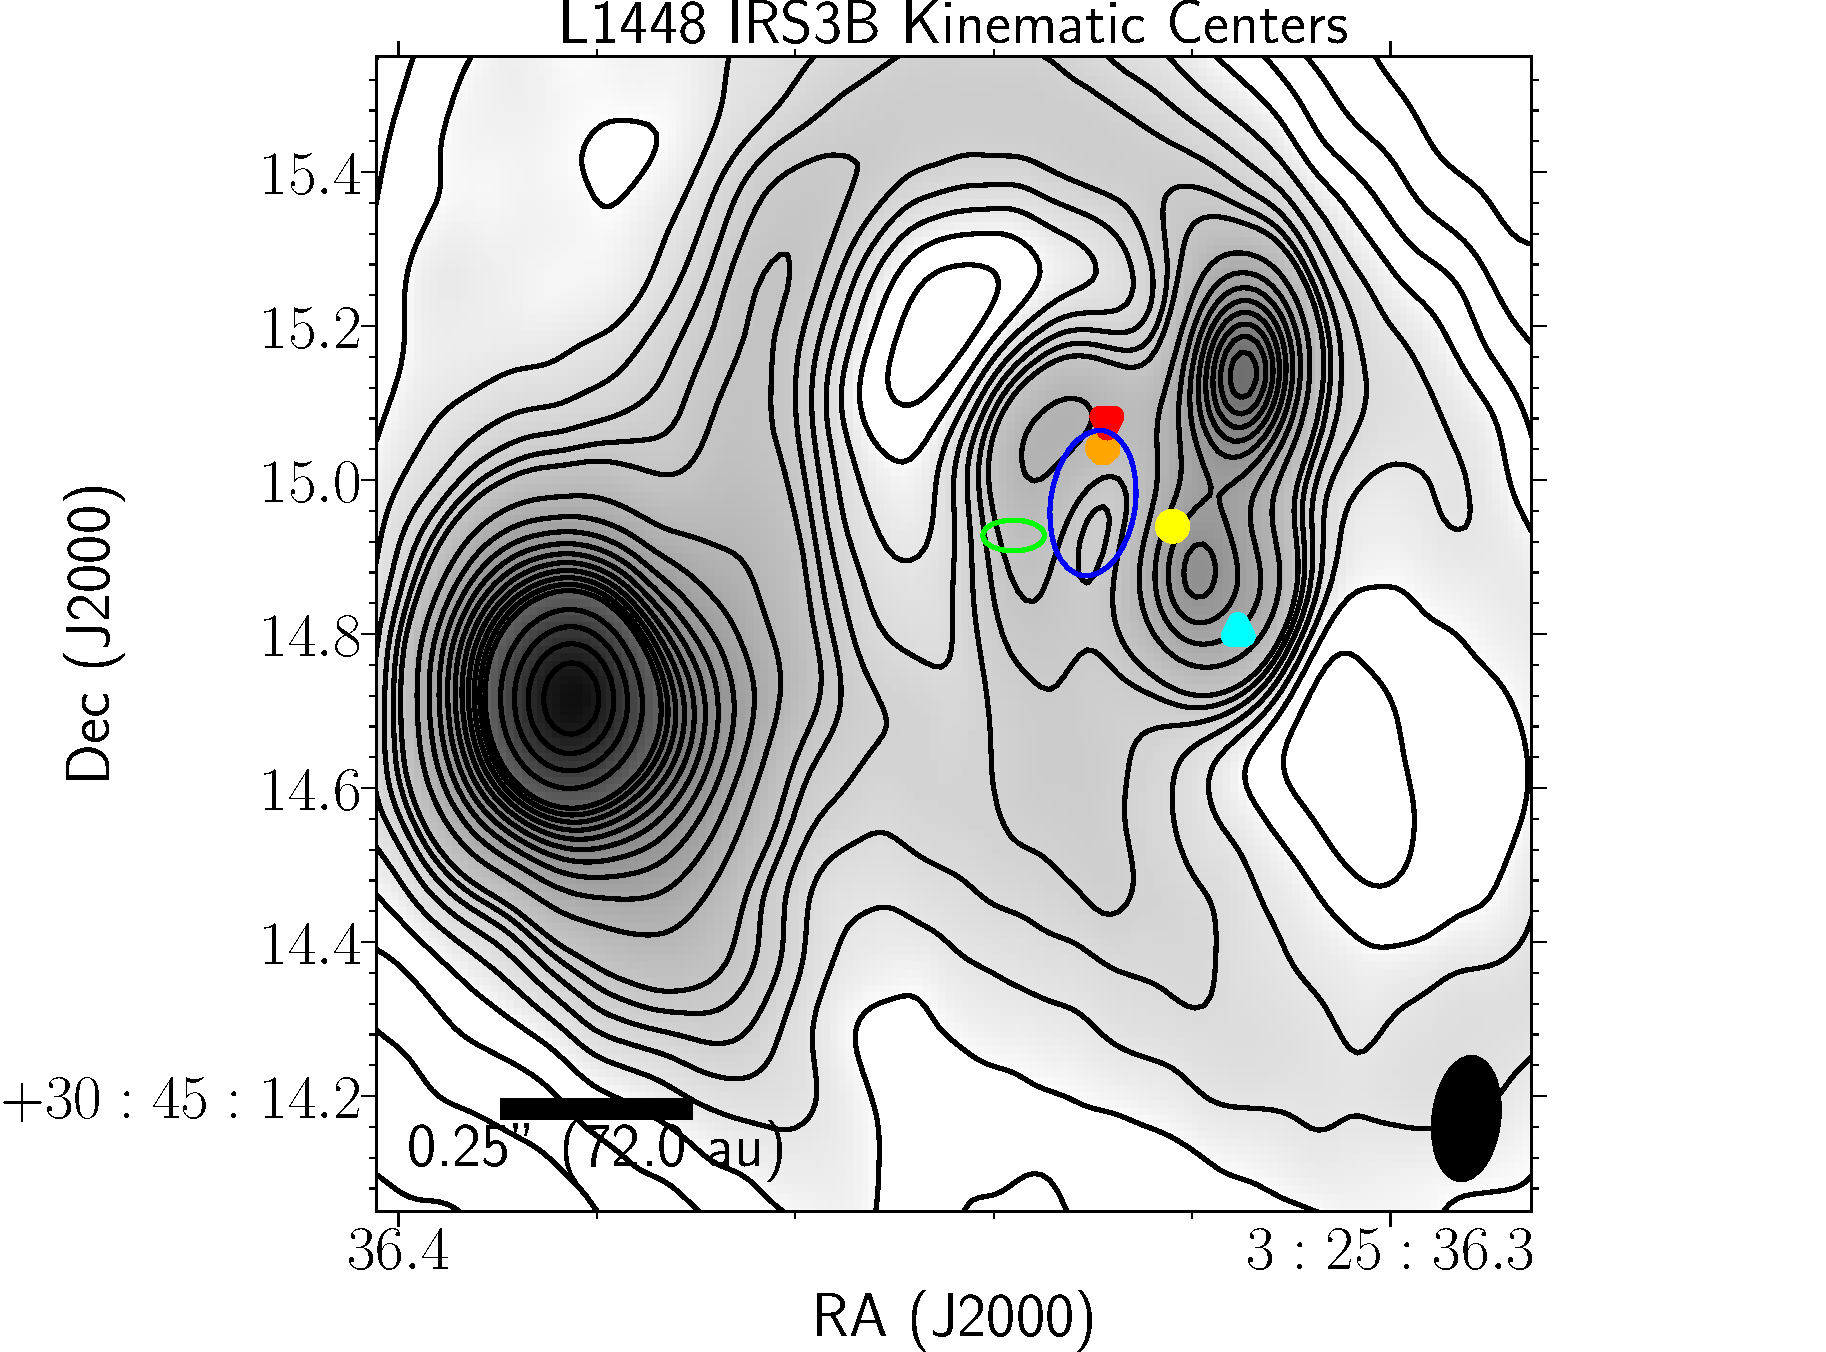
\includegraphics[width=0.48\textwidth]{img/L1448IRS3B_cont_robust05kincenters_zoom.pdf} % h13cn
\end{center}
   \caption{Positions of the various ``kinematic centers'' that have been fit from \cso\space emission at IRS3B in relation to continuum structure. The grayscale is the dust continuum from Figure~\ref{fig:zoomincont}. Left: The red colored texts detail the locations of continuum sources, presumed to be protostars. Right: A zoom in on the region indicated by the black rectangle in the left image. The red and blue triangles indicate the central Gaussian fit of the highest Doppler-shifted velocity emission with the yellow circle indicating the midpoint. The orange circle indicates the center that best constructs the PV diagram symmetrically. The green ellipse is the model Keplerian centroid fit with the respective error as indicated by the size of the ellipse (see Section~\ref{sec:kmodelresults}). The blue ellipse is the \cso\space beam (\csobeam) centered on the region of emission deficit for size comparison. The contours start at 10$\sigma$\space and iterate by 10$\sigma$\space with the 1$\sigma$~level starting at 8.5$\times10^{-5}$~Jy~beam$^{-1}$. The region of deficit, first identified in Figure~\ref{fig:zoomincont}\space is shown to be centered within the three various kinematic center fits and are marginally separated by less than a few beams.}\label{fig:kincenter}
\end{figure}




% figure 17 here

% Figure 16
\begin{figure}[H]
\begin{center}
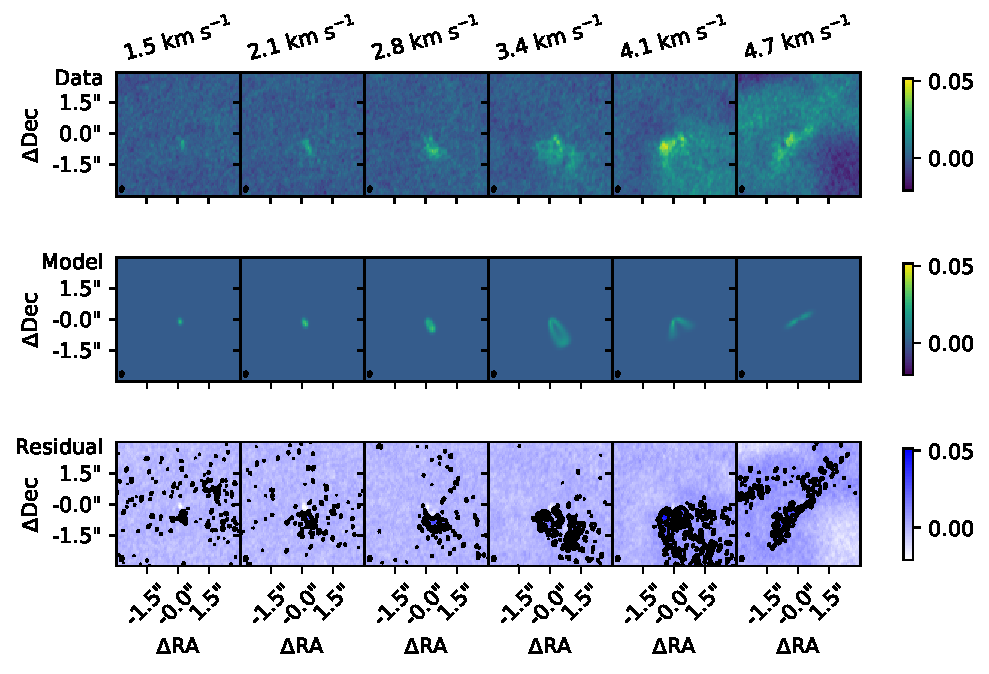
\includegraphics[width=0.49\textwidth]{img/Channelplot_irs3bplotblue_C17O.pdf}
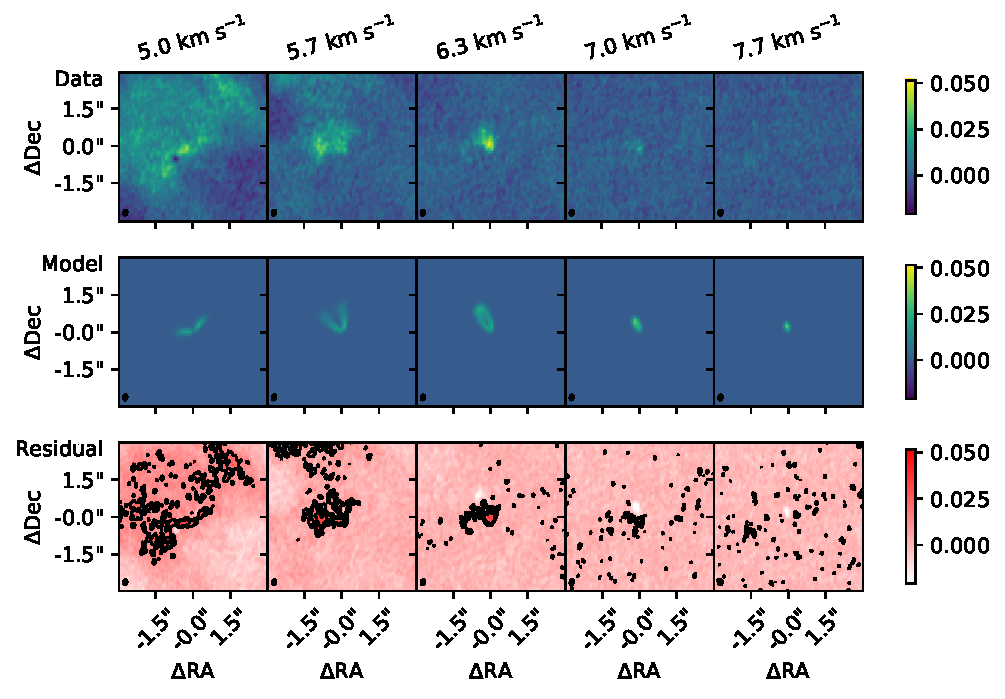
\includegraphics[width=0.49\textwidth]{img/Channelplot_irs3bplotred_C17O.pdf}
\end{center}
\caption{IRS3B Kinematic Model: A representative selection of channel maps that fit the model to the data. The left figure is the blue Doppler shifted emission while the right figure is the red Doppler shifted emission. The first row contours are the model contours, generated at the 2, 3, 5, and 10$\sigma$ level overlaid the data channels selected at the same velocity. The second row is the residual contours (2 and 3$\sigma$) overlaid the same data channels. System velocity is \ab4.8~km~s$^{-1}$. It should be noted the highly correlated structure visible in the residuals. This reflects an imperfect fit to the data given that the circumstellar disk itself is asymmetric.}\label{fig:c17o_res}
\end{figure}



% figure 21
\begin{figure}[H]
\begin{center}
%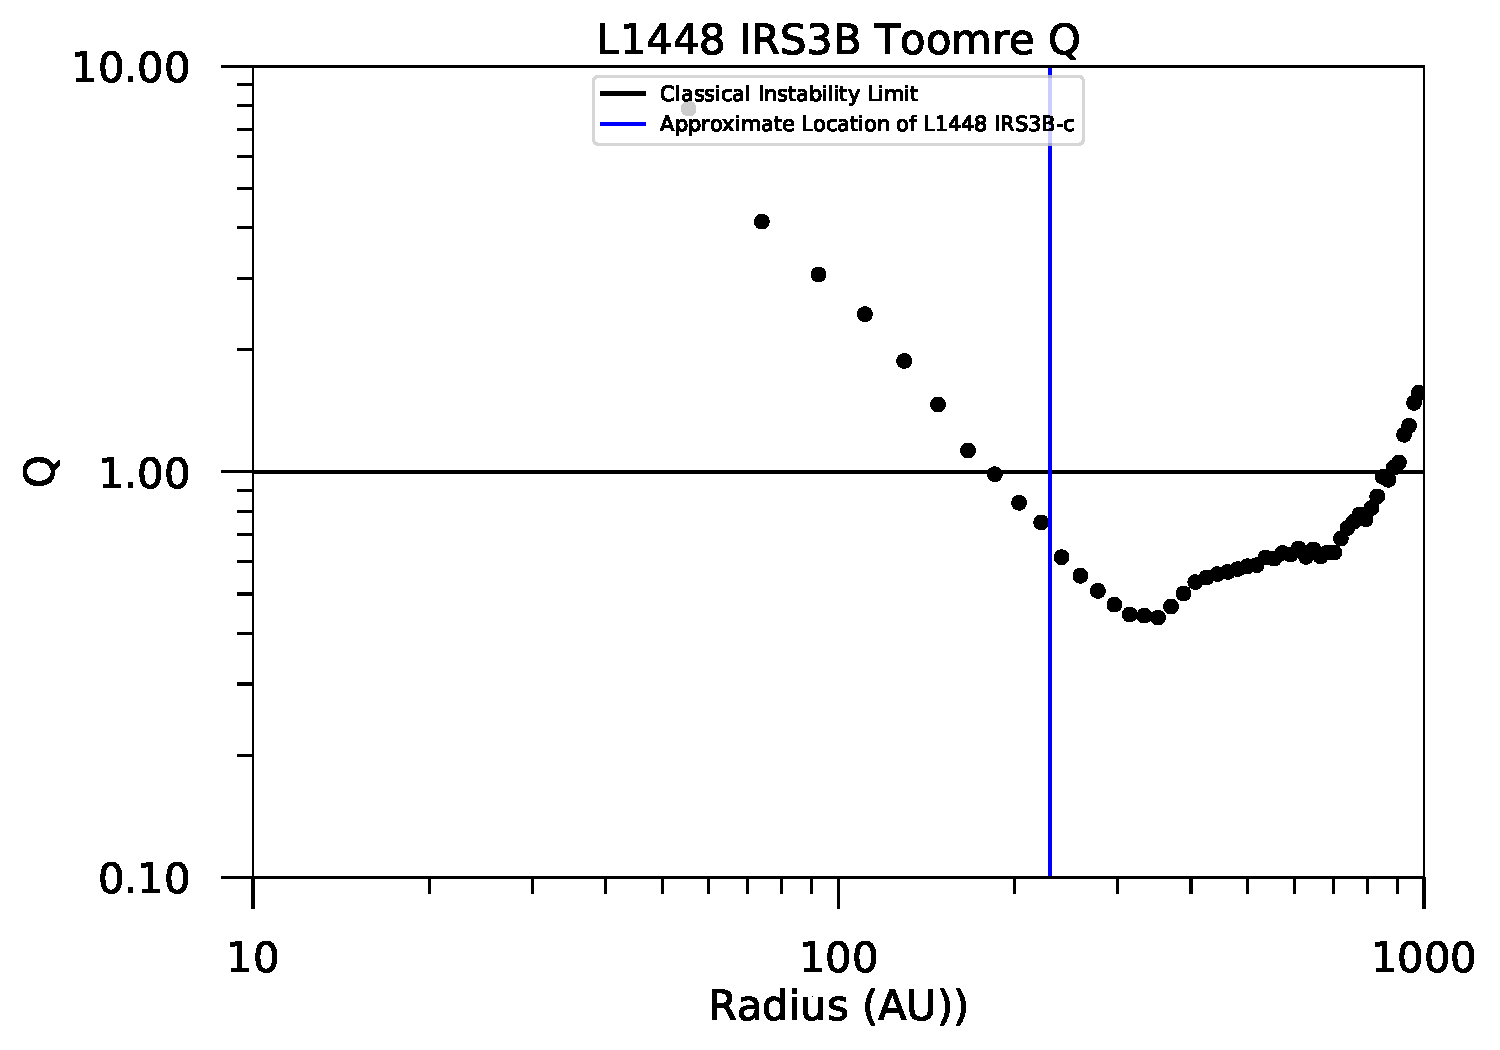
\includegraphics[width=0.48\textwidth]{img/L1448N-toomre-Q-linear-xsec-c17o_cont.pdf}
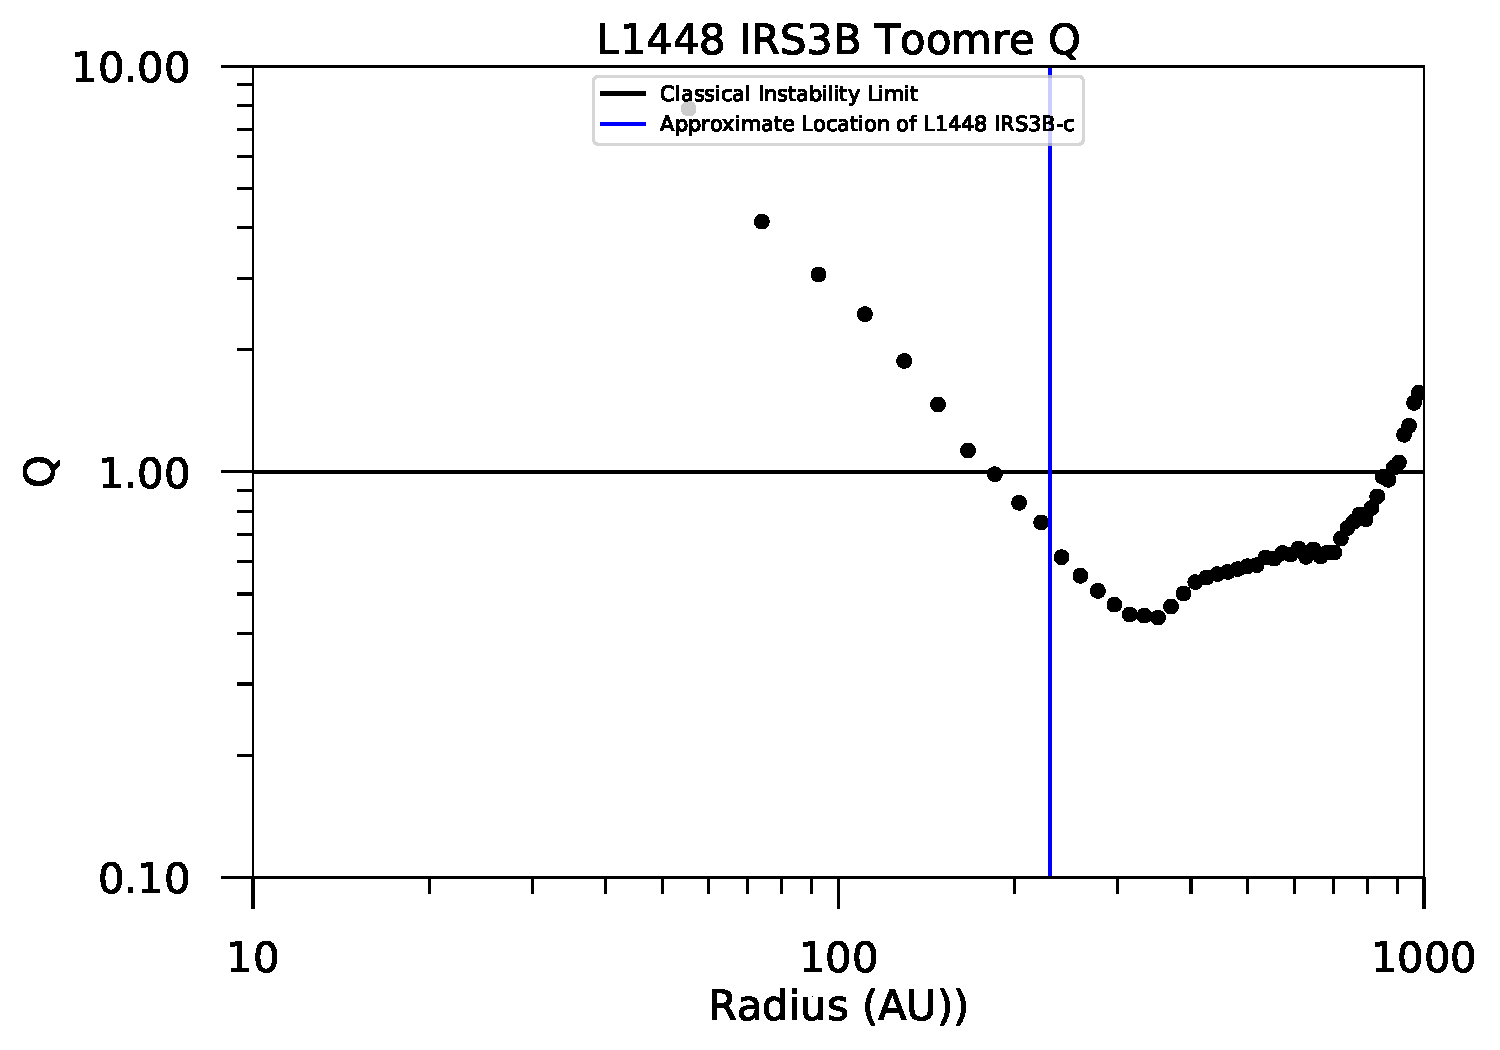
\includegraphics[width=0.49\textwidth]{img/L1448N-toomre-Q-linear-xsec-c17o_cont.pdf}
%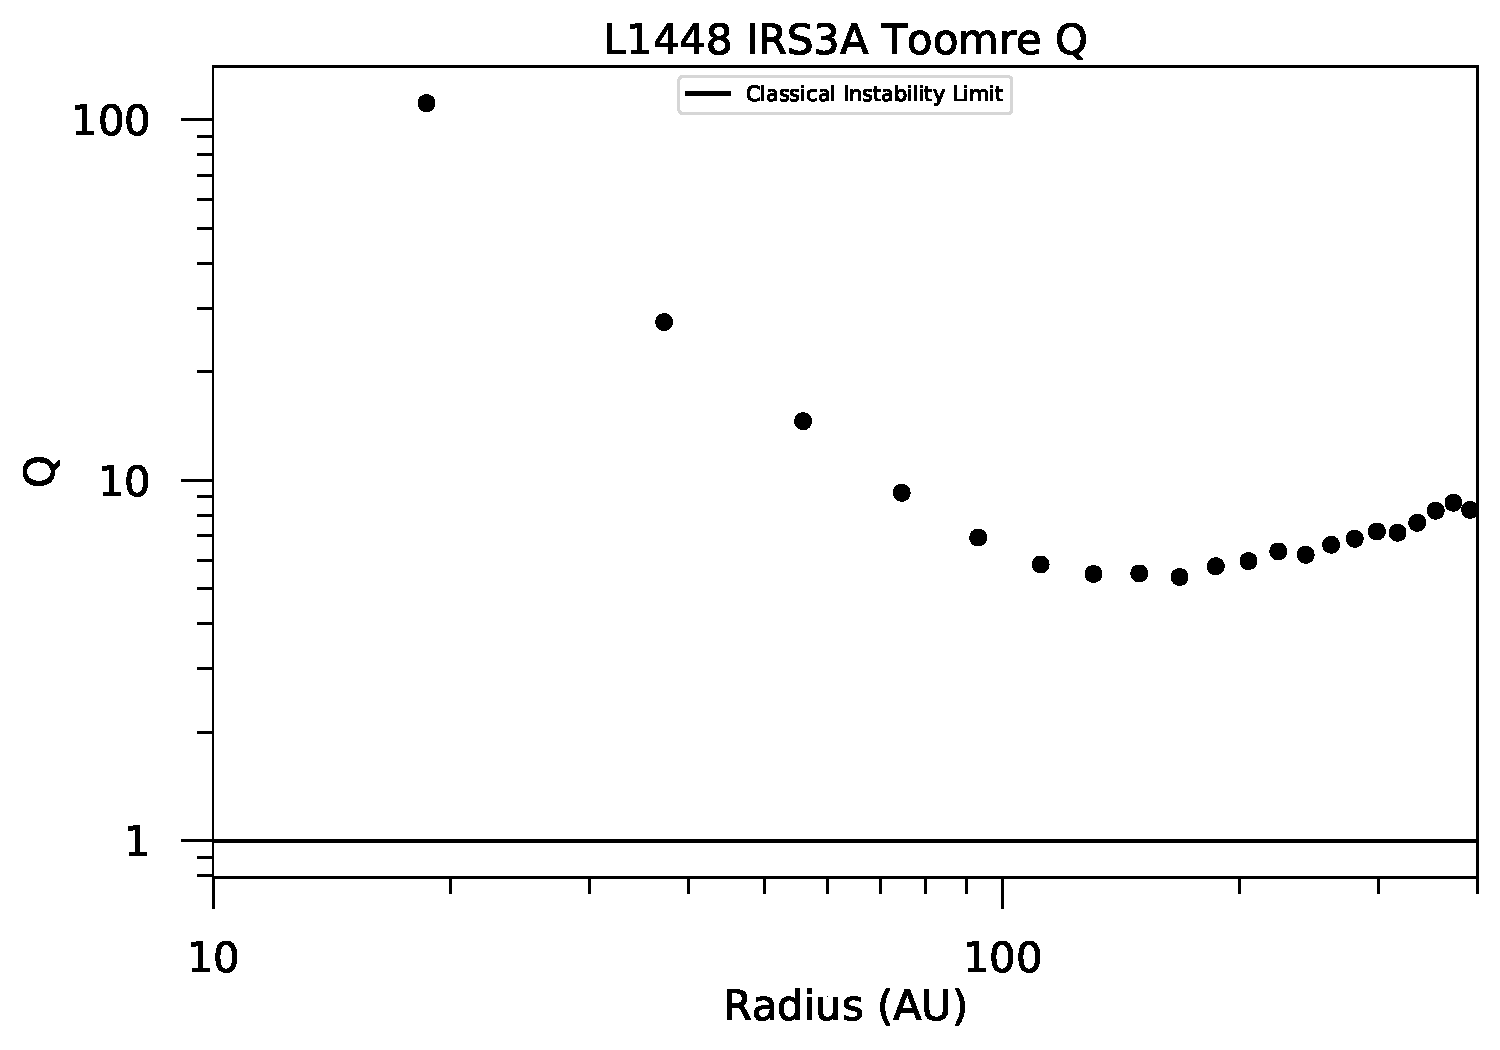
\includegraphics[width=0.49\textwidth]{img/L1448N-toomre-Q-linear-xsec-cont_robust-05_wide.pdf}
\end{center}   
\caption{Toomre Q parameter plotted as a function of deprojected radius for IRS3B (left) and IRS3A (right). The horizontal line indicates a Toomre Q parameter of one, at which the disk would be gravitationally unstable. As indicated, the IRS3B disk Toomre Q parameter drops below 1 at a radius of \ab120~AU. The vertical line corresponds to the deprojected radius of IRS3B-c. The observed spiral arms also become most prominent at R $>$100~AU, where Toomre~Q approaches 1. The circumstellar disk of IRS3A is much less massive than IRS3B, coupled with a more massive protostar, the disk is more stable against gravitational instabilities.}\label{fig:irs3btoomreq}
\end{figure}



% -----------------------------
% backmatter
\clearpage

% bib
{
\begin{tiny}
\cftaddnumtitleline{toc}{section}{}{References}{\thepage}
\bibliographystyle{apj}
\bibliography{main}\label{sec:references}
\end{tiny}
}

% glossary
{
\cftaddnumtitleline{toc}{section}{}{Glossary}{\thepage}
\printnoidxglossary\label{sec:glossary}
\printnoidxglossary[type=\acronymtype]
}
% appendex
\end{document}
